% Based on the ACM SIG Proceedings sample. The KDD Research CFP specifies
% sigconf,anonymous,review. Overleaf root document: main.tex.
% The original vector overview is PDF 1.7.
\ifdefined\pdfminorversion\pdfminorversion=7\relax\fi
\documentclass[sigconf,anonymous,review]{acmart}
\setcopyright{none}
\acmDOI{}
\acmISBN{}
\acmConference[KDD 2027 Research Track]{KDD 2027 Research Track}{August 2027}{San Jose, CA, USA}
\acmBooktitle{Manuscript prepared for the KDD 2027 Research Track}
\acmYear{2027}
\usepackage{amsmath}

\begin{document}
\title[Which Analyses Can Agent-Generated Cohorts Support?]{Which Scientific Analyses Can Agent-Gener\-ated Biomedical Cohorts Support?}
\author{Anonymous Author(s)}

\begin{abstract}
Biomedical studies often publish results for individual measurements while withholding the paired records needed for a new analysis. We study scientific agents that turn these summaries into sampling programs. We isolate one modeling decision by holding every measured value in a virtual cohort fixed and changing which values belong to the same person. In a Chinese community holdout, restoring the six agents' original iron-status pairings improved correlation accuracy in every case. Four other agents produced lipid models that matched the same published summaries yet differed in screening prevalence by 16.37--29.35 percentage points within author. In a prospective test on 3,857 US and South African adults, four agents given only Australian summaries for each hand independently chose the same dependence model. Their virtual mean absolute difference between hands was 3.81 kg, versus 3.30 and 3.78 kg measured. Independent pairing of identical values gave 7.93 kg. Yet the same virtual records overestimated South African mean grip strength by 7.81 kg. Testing each analysis separately reveals where an agent's modeling decision supplies a useful missing relationship and where a population's marginal measurements still limit the result.
\end{abstract}

\ccsdesc[500]{Computing methodologies~Modeling and simulation}
\ccsdesc[300]{Applied computing~Life and medical sciences}
\keywords{scientific agents, synthetic biomedical data, joint distributions, evidence synthesis, analysis utility}
\maketitle

\begin{figure*}[t]
\centering
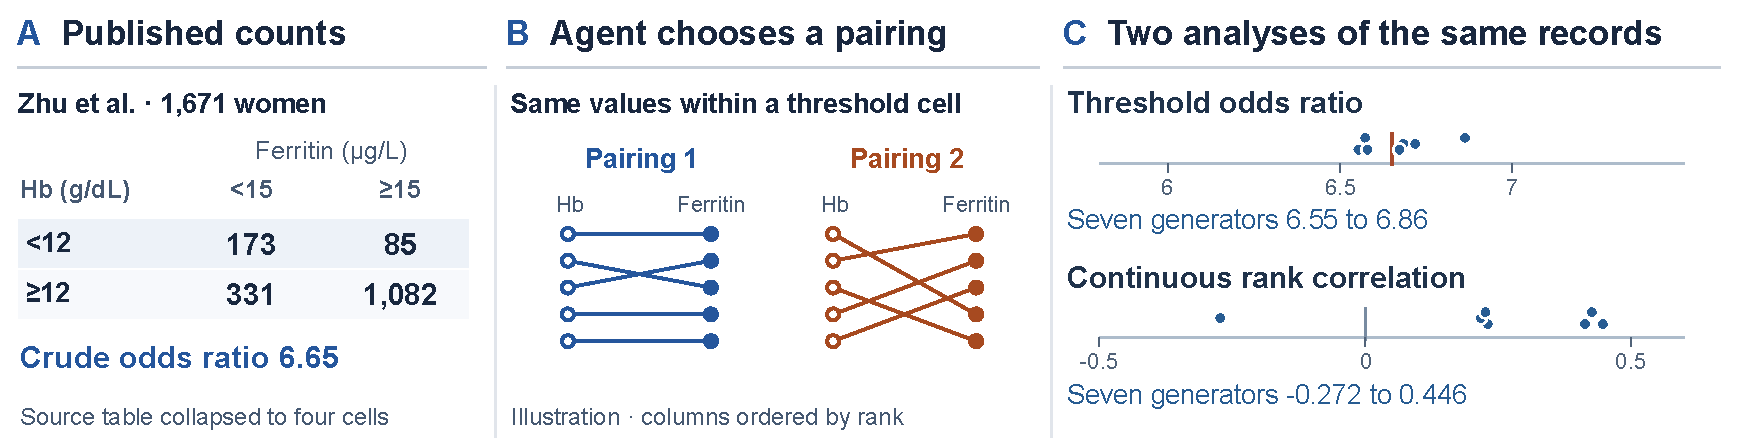
\includegraphics[width=\textwidth]{figures/evidence-and-pairing.pdf}
\caption{From a published summary to paired virtual records. (A) Collapsing the iron-status groups in Zhu et al.~\cite{zhu} yields four counts and a crude anemia odds ratio (OR) of 6.65 for low versus higher ferritin. (B) The lines illustrate two ways of assigning the same five ferritin values to the same five hemoglobin values in one threshold cell. Either assignment preserves the cell count. (C) Seven programs that passed the source checks produced similar threshold ORs and a wide range of continuous Spearman correlations. Each dot is one program. The orange mark gives the source OR. The models see the reported band summaries as well as the counts.}
\Description{A two-by-two table implies an odds ratio of 6.65. Two illustrative matchings preserve the values assigned to the cell. Seven real program outputs give odds ratios from 6.55 to 6.86 and continuous correlations from minus 0.272 to 0.446.}

\label{fig:method}
\end{figure*}

\section{Introduction}
A researcher wants to compare urban and pastoralist adults after adjusting for age and sex. She has a paper describing both groups, but she cannot obtain its individual records. A scientific agent can read the reported summaries and generate a table with one row per person. Can she use that table for the same BMI and cholesterol regressions she would have run on measured records? An error of one unit has a different meaning across the two outcomes. Even two samples of real participants can return different estimates.

The scientific choice is clearest when a study reports two measurements in groups. A paper on anemia in northern China tabulates iron, folate and vitamin B$_{12}$ status~\cite{zhu}. Four collapsed counts already determine the source odds ratio for low hemoglobin and low ferritin. They leave open which continuous ferritin value belongs with each hemoglobin value inside a cell. That choice can change a rank correlation while preserving every count (Figure~\ref{fig:method}). A further question arises when a researcher applies that choice to another population.

Previous work generates synthetic cohorts from shared fitted models, aggregate statistics, trial curves and published covariates~\cite{filshtein,llmsynthor,synthipd,kmgen}. We evaluate one requested analysis in one population at a time. Its unit of evaluation is a scientific estimate, such as an adjusted group contrast or the proportion crossing a laboratory threshold. Our three contributions follow that estimate from the paper into the data.
\begin{enumerate}
\item \textbf{Trace what the source determines.} We link each reported number and its arithmetic implications to the measurement, population and role it has in the executable generator.
\item \textbf{Isolate the agent's pairing decision.} We alter which measurements share a person, hold their values fixed, and recompute the same analysis. We also give independent agents a source paper's lipid summaries and ask each for two executable models. Their screening rates quantify the consequences of their own modeling choices.
\item \textbf{Test each scientific use on measured records.} We compare estimates against real-sample variation and seal the planned analyses before opening new samples. We test the same lipid models across populations and periods. In a prospective handgrip study we use two recruitment settings to test the agent's choice against both measured individuals and a statistical model given the same evidence.
\end{enumerate}

\section{From a research request to executable records}
\label{sec:method}



\paragraph{Scientific contract.}
A request names the unit of observation, population, measurement units and intended analyses. For example, the iron request calls for continuous hemoglobin and ferritin in nonpregnant US women aged 20--44. We disclose the analyses to the constructor so it can seek appropriate evidence. The measured target records and their analysis results stay with the evaluator. All experiments here generate whole records. Figure~\ref{fig:method} follows one such construction from its source counts to two group analyses. In the community holdout, constructors also see tables newly calculated in the evidence communities. Individual measurements from either half remain unavailable to them.

Write $s_j(P_j)$ for a statistic evaluated under the population, measurement and adjustment rules of source study $j$. A paper reports a rounded estimate of this quantity. The researcher's question is an analysis $a(P_T)$ in target population $T$. Even exact knowledge of $s_j(P_j)$ generally leaves open both the shape of the source distribution and the correspondence between $P_j$ and $P_T$. We use this distinction in two ways. We compare a generated estimate of $a$ with the same estimate in a measured sample. Where source summaries permit several laws, we can also ask whether varying the law changes $a$ while preserving those summaries.

\paragraph{Agent and execution service.}
In the initial original-paper experiments (Section~\ref{sec:original}), each fresh model session received a starting paper, the request, tools for reading and supplementary retrieval, an output schema and an execution budget. The agent could inspect source tables and methods, resolve units, propose a dependence structure, and choose numerical parameters. It returned an executable sampler, its parameters and a record of consequential choices. It could inspect a trial draw and submit a revision. The execution service validated the interface, ran the submitted program in isolation and recorded its identity and seeds. The coordinator supplied the task and starting article. The constructor selected the scientific law. The final rows were sampled from that law. The study therefore tests authorship of a reusable generator from an assigned paper. Each of the two articles was assigned to three sessions.

\paragraph{Audit of a modeling decision.}
For each quantity we record what the source reported, how the agent transformed it and how the code used it. We separately record any change of population or statistical definition. For example, a partial correlation can be exactly derived from a source matrix while its use as a residual correlation after additional adjustment remains an assumption. We check the submitted program against the account of the model choice and independently recompute scientific estimates. This audit can establish that a model implements its stated choice. Only evidence on the requested analysis can establish how useful that choice was.

\paragraph{Evaluation.}
Each constructor commits its program before the final draws. Draws with different seeds measure variation conditional on that program. Separate constructors can express different modeling choices. For each task we run a single estimator implementation on generated records and the measured reference under the relevant sampling design. For the published lifestyle analysis, this is a reimplementation of the reported regression. A reference value estimates a quantity in a measured sample and carries uncertainty. The community holdout specifies planning tolerances and a minimum worthwhile change before generation. Elsewhere we report discrepancies in native units. All scores here describe group analyses. We did not evaluate individual-level prediction.

\section{Re-running the published lifestyle analysis}
\label{sec:lifestyle}
Lea et al. compared lifestyle groups among Turkana adults in Kenya~\cite{lea,leadata}. Two agents independently wrote generators from the study evidence, each yielding three tables with age, sex, lifestyle, BMI and blood lipids. We reimplemented the age- and sex-adjusted contrasts once and changed only the input table. This is same-study reconstruction: the publication and measured reference describe the same study. Published group information is available to the agent.

\begin{figure*}[t]
\centering
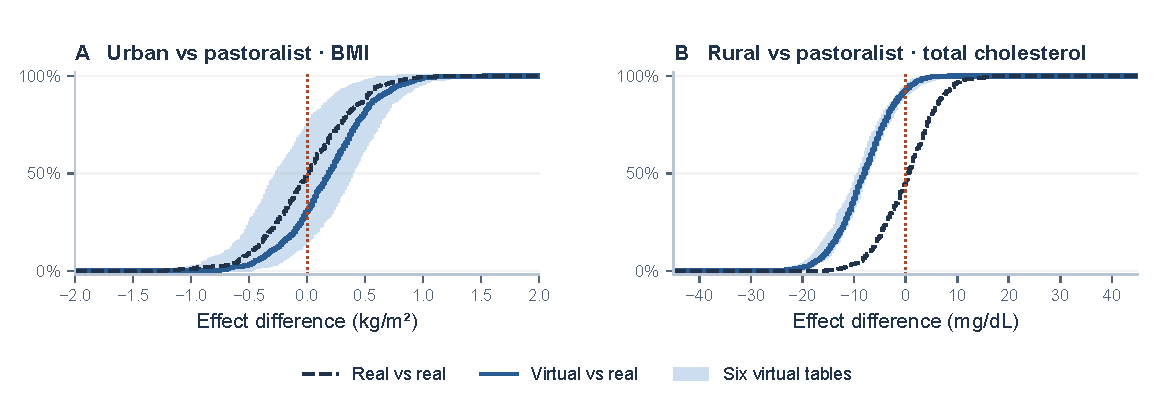
\includegraphics[width=.91\textwidth]{figures/lifestyle-main.pdf}
\caption{How large is a discrepancy between two analyses? Each curve gives the fraction of 500 matched resamples with an effect difference at or below the horizontal value. The dashed line compares two real resamples. Blue compares virtual with real; the solid curve is the pointwise median and the band spans six fixed virtual tables from two constructors. In (A) urban BMI discrepancies are on the scale seen between real resamples. In (B) the virtual rural cholesterol contrasts tend to be smaller. Appendix Figure~\ref{fig:lifestyle} and Table~\ref{tab:lifestyle} retain all nine comparisons.}
\Description{Cumulative curves overlap for the urban versus pastoralist BMI contrast. The virtual-versus-real curves shift left for rural versus pastoralist total cholesterol.}
\label{fig:lifestyle-main}
\end{figure*}

In each of 500 repetitions we drew two real samples and one sample from each virtual table, with the same size and sex-by-lifestyle composition for each trait. For urban versus pastoralist BMI, real resamples differed by 0.316 kg/m$^2$ on average in absolute value. Virtual--real discrepancies ranged from 0.314 to 0.428 kg/m$^2$ (Figure~\ref{fig:lifestyle-main}A). For rural versus pastoralist total cholesterol, generated data understated the adjusted effect by 7.80--9.54 mg/dL on average (B). The corresponding HDL effects were low by 4.07--6.21 mg/dL. Total and HDL cholesterol SDs in the measured sample were 42.81 and 20.23 mg/dL; virtual resampling gave 31.49--32.67 and 14.50--14.89. The urban BMI analysis is supported as a rehearsal at this scale. The same tables would understate lipid variability in a study-planning calculation. These resamples describe one study and do not establish equivalence in a new population.

\section{Can the agent model what the paper reports?}
\label{sec:original}


We ran three fresh sessions on each of two requests using the same recorded GPT configuration. All six located the relevant table in the assigned original article, performed a numerical derivation, authored a whole-cohort generator, inspected one simulated trial and retained the first candidate. Each law produced three final draws. The 18 tables contain 72,000 simulated records. Independent computation reproduced all 99 draw-level analysis and diagnostic estimates to within $7.6\times10^{-14}$. Construction used 142 model calls at an estimated token tariff of US\$1.51. These counts describe six modeling decisions.


\paragraph{Blood pressure.}
The assigned article studied partnered adults aged at least 40 in rural Burkina Faso~\cite{jaspert}. Its correlation matrix gives the associations of age, body mass index (BMI), systolic blood pressure (SBP) and diastolic blood pressure (DBP). Each agent combined its entries to obtain the source age- and BMI-adjusted residual correlation, approximately 0.788. The source also reports BMI regression coefficients from a more extensively adjusted model. The agents used positive diastolic and pulse pressures and summed them to obtain systolic pressure. They chose different demographic distributions and conditional pressure levels. This construction enforces the physical ordering of the two pressures for every draw.

We applied the target regressions to virtual records and compared them with estimates from 8,352 eligible participants in the Brazilian National Health Survey (PNS)~\cite{pns}. The age- and sex-adjusted systolic slope ranged from 3.40 to 3.80 mmHg per five BMI units, bracketing the measured 3.52. The corresponding diastolic slopes were 2.29--2.40 versus 2.26. The pressure correlation after adjusting for age, sex and BMI was 0.772--0.781 versus 0.717. All three laws also yielded wider pressure distributions than the measured sample (Appendix~\ref{app:profiles}). Thus a user could recover the direction and approximate scale of these BMI associations while overestimating dependence between the paired measurements.

\paragraph{Iron status.}
Of the women in the source table, 173 had both markers low, 85 had only low hemoglobin, 331 had only low ferritin and 1,082 had neither~\cite{zhu}. Each agent computed the crude odds ratio, $(173\times1082)/(85\times331)=6.65$, and distinguished it from the paper's adjusted odds ratio of 6.448. One agent then used a Clayton copula to couple continuous biomarker values. Another modeled two latent iron-store components and a change in hemoglobin response below a threshold. The third used a saturating response with inflammatory and other-anemia components. Supplementary evidence informed marginal assumptions. All three authors noted an ambiguity in the source's ferritin labeling.

We evaluated crude threshold odds, joint prevalence and rank correlation against survey-weighted US National Health and Nutrition Examination Survey (NHANES) estimates from 979 eligible women~\cite{nhanes}. The thresholds were hemoglobin $<12$ g/dL and ferritin $<15$ $\mu$g/L. Generated odds ratios were 6.35--7.14, close to the source's 6.65. The measured US odds ratio was 17.79. All three programs preserved a positive association and substantially understated its strength in this comparison. For the same records, the prevalence of both low markers was 4.67--5.85\% versus 7.63\%, and Spearman correlation ranged from 0.197 to 0.329 versus 0.398 (Figure~\ref{fig:original}). A correct table extraction can therefore coexist with appreciable error after population transfer.

\paragraph{What does direct arithmetic already give the researcher?}
Five times the published BMI coefficients gives 3.75 mmHg for SBP and 2.20 mmHg for DBP in the source's fully adjusted model. Those two numbers provide informative comparisons with the Brazilian slopes, even before simulation. Likewise, the four iron counts yield the crude odds ratio and a joint-low prevalence of 10.35\% for the Chinese study. They supply no continuous rank correlation. For that question, choosing how to populate the four cells with continuous values is the scientific modeling step. Comparing the three authored programs makes that choice visible.

\section{What changes when the agent gets joint evidence?}
\label{sec:controlled}
We held the research request and modeling interface fixed within each task and changed the supplied evidence. Three fresh constructors worked in each of three conditions per case, with three final seeds per constructor. The first condition provided the common base. For pressure, this already contained previously published relationship evidence. For iron status, it supplied study context. The second condition added single-variable summaries from the selected source. The third added a joint block \emph{from the same source sample}. This consisted of six pairwise correlations for pressure, or the paired low-marker counts for iron. The latter two conditions differed only in that block. No target feedback or programmed numerical relationship entered these comparisons.

\begin{table}[t]
\caption{Mean absolute discrepancy by evidence condition. The last two columns differ only in the joint source block. Lower is closer to the measured sample within each row.}
\label{tab:evidence}
\centering
\begin{tabular}{@{}lrrr@{}}
\toprule
Requested analysis & Base & Marginal & Joint\\
\midrule
BP residual correlation & .1632 & .1633 & \textbf{.0350}\\
BMI--SBP slope & .1934 & .3396 & .5091\\
BMI--DBP slope & .7276 & .7378 & .7550\\
Iron log odds ratio & 1.5495 & 1.7620 & \textbf{.9373}\\
Both markers low (pp) & 1.7903 & .5187 & 2.5940\\
Iron rank correlation & .0769 & .0447 & .1736\\
\bottomrule
\end{tabular}
\end{table}

Table~\ref{tab:evidence} reports discrepancies for every requested analysis. We computed the absolute error for each draw and averaged first across seeds, then equally across constructors. The two pressure slopes are in mmHg per five BMI units. The iron odds ratio is evaluated on the natural-log scale. Adding the matrix reduced residual-correlation error from 0.1633 to 0.0350. Adding the four-cell table reduced log-odds-ratio error from 1.7620 to 0.9373. The two other pressure estimates and the two other iron estimates moved farther from their respective sample references. In particular, the joint table identifies a threshold association in its source sample but gives neither the target prevalence nor the within-cell ordering needed for continuous ranks. These results identify the change across the tested evidence conditions. Their magnitude is descriptive across three constructors per condition.

\section{Can the same pressure moments predict joint screening?}
\label{sec:prospective}
A Burkina Faso study supplied five blood-pressure moments~\cite{jaspert}. One agent wrote two laws that preserved the source correlation of 0.78 and implied joint blood-pressure screening rates of 11.94\% and 15.09\%. The simulated difference missed its prespecified margin after allowing for sampling noise. In Freetown 44.21\% of 1,244 eligible records crossed both cutoffs. None crossed only one. The deposited component fields have an unresolved pairing history, which limits the biological interpretation~\cite{freetown,freetowndata}. Appendix~\ref{app:freetownaccount} gives the complete prospective comparison.

\section{Which iron analyses survive a change of model?}
\label{sec:ironpros}
Three agents read the full Chinese article~\cite{zhu} and proposed iron-status generators. Further sessions proposed alternative laws under the same evidence. All seven completed programs passed the 16 source checks. Their low-ferritin anemia odds ratios clustered near the 6.65 implied by the published counts. Their continuous correlations ranged from $-0.272$ to $0.446$. With 44 measured mothers in rural Burkina Faso~\cite{burkina_iron}, the rank estimate was 0.069 (95\% interval $-0.198$ to $0.389$). None had low ferritin, so their threshold odds ratio could not be estimated. Figure~\ref{fig:method} and Appendix~\ref{app:ironpros} identify the pairing decisions and the four completed primary--alternative comparisons.

\section{Can the same virtual cohort support two held-out iron analyses?}
\label{sec:chns}
The external Burkina Faso sample had too few low-ferritin observations to evaluate the threshold analysis. For a test with information from the target population, we used the 2009 China Health and Nutrition Survey (CHNS)~\cite{chnsbio,chnsind}. We split whole communities within nine provinces before scoring. The evidence half (A) comprised 1,123 women in 110 communities. The held-out half (B) comprised 1,082 women in 107 other communities. All were aged 18--49 with paired central hemoglobin (Hb) and serum ferritin measurements. The halves shared no people, households or communities. The survey family had been used in development. The partition and its iron endpoint were new.

\paragraph{An identical starting point for each pair of revisions.}
Three ordinary coding agents and three agents given scientific modeling guidance used the same GPT configuration. Each received the Zhu article and two tables newly computed from A, one reporting joint threshold counts and the other summarizing ferritin by Hb band. Each chose its own law and parameters. Two further sessions independently reviewed each sealed law with the same feedback on its generated records and the original evidence. Only one received a new A statistic. Within Hb 12--$<14$ g/dL, geometric mean ferritin was 1.215 times as high at Hb 13--$<14$ as at 12--$<13$ g/dL (95\% interval 1.061--1.398). Neither branch received a whole-cohort rank correlation. We sealed all programs and outputs before opening B.

\paragraph{Final utility on the two prespecified analyses.}
We ran the same unweighted rank and threshold estimators on virtual and measured records. B's Spearman correlation was 0.317 (95\% community-bootstrap interval 0.259--0.373). All six augmented laws gave 0.297--0.304, within the prespecified absolute tolerance of 0.10. For low Hb ($<12$ g/dL) comparing low ferritin ($<15$ $\mu$g/L) with higher ferritin, the six crude odds ratios were 4.990--5.124. B's estimate was 4.218 (2.979--6.042). All six preserved the positive threshold association and met the factor-of-1.50 tolerance, while overstating its magnitude by 18--22\%. The A threshold table already implied an odds ratio of 5.083. The global rank analysis tests a relationship absent from the supplied tables. Both conclusions concern planning with these measured populations.


\paragraph{What does the agent add to the original evidence?}
After B was disclosed, we specified one statistical comparator that fits the A band sizes, Hb moments, ferritin geometric moments and depletion frequencies. It draws Hb and ferritin independently within each of the three reported Hb bands (Appendix~\ref{app:chnsstat}). It met both original target-comparison margins. Its pooled rank was 0.2370 (analytic population value 0.2414). All six original-evidence agent laws gave ranks closer to B (Table~\ref{tab:chnsattribution}). To isolate the contribution of pairing while keeping each agent's own bandwise marginals, we computed its expected rank after randomly re-pairing the two biomarkers within each band. Restoring the authored pairs reduced absolute rank error for all six, by a median of 0.0612. The threshold odds ratio was exactly invariant to this change. This localizes the improvement to an aspect of the model the A tables leave open. Its size is relative to the measured estimate on this split.

\begin{figure*}[t]
\centering
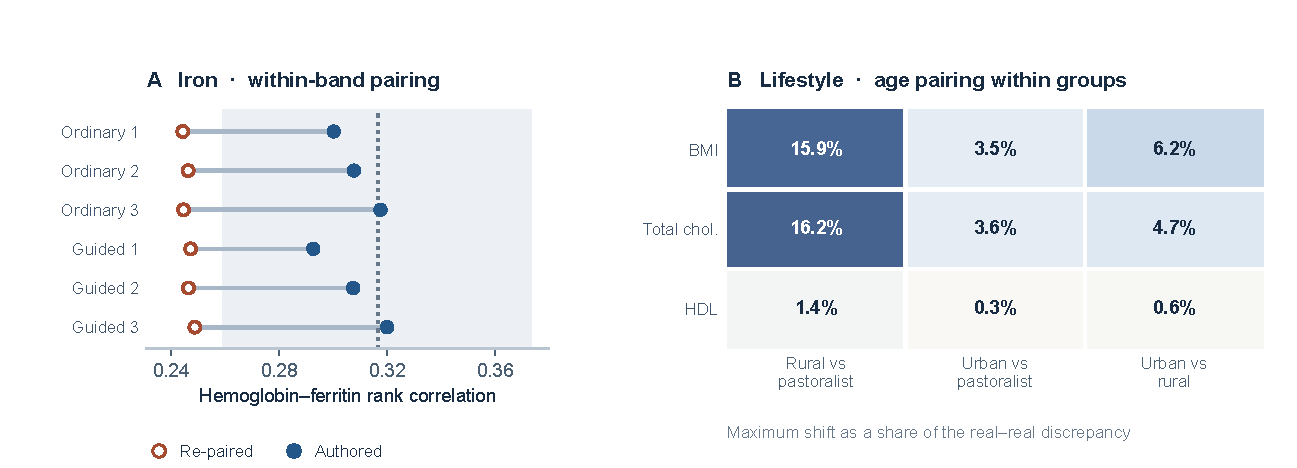
\includegraphics[width=.94\textwidth]{figures/pairing-attribution.pdf}
\caption{How much of an analysis comes from the agent's pairing? (A) Each line follows one CHNS law from the expected correlation after randomly re-pairing within Hb bands to its authored value. The dotted line and shading show the measured correlation and its 95\% interval. (B) In the lifestyle case, age was re-paired with the intact biomarker vector within sex and lifestyle groups. The cells show the largest absolute change over all six virtual tables as a percentage of the mean absolute difference between two real resamples for that regression. These are retrospective within-table comparisons.}
\Description{All six authored iron correlations lie closer to the measured sample than their re-paired counterparts. The largest age-pairing shift for the nine lifestyle regressions ranges from 0.3 to 16.2 percent of the corresponding real resampling discrepancy.}
\label{fig:attribution}
\end{figure*}

The lifestyle example provides a comparison where pairing did little (Figure~\ref{fig:attribution}B). In each of its six virtual tables, we kept every outcome vector and randomly reassigned it among participants in the same lifestyle and sex group. The expected age-adjusted urban--pastoralist BMI contrast moved by only 0.0025--0.0110 kg/m$^2$. The real--real mean absolute difference was 0.316. The group structure already supplied most of this particular contrast. Across all nine regressions the largest shift reached 16.2\% of the corresponding real--real difference. Appendix~\ref{app:pairingtest} gives the calculation.



Five of six revisions improved agreement with the supplied within-band ferritin contrast. Only one improved held-out whole-cohort rank accuracy. The largest control error was already 0.024, below the prespecified improvement of 0.05. A retrospective decomposition showed that other bands accounted for most of the measured correlation (Appendix~\ref{app:chns}, Figure~\ref{fig:revision}).

\paragraph{A prospective comparison in a new cohort.}
Before computing either endpoint in the Akwa Ibom survey in Nigeria~\cite{akwa_iron}, we fixed a comparison that isolates the pairing decision. All methods received the same Chinese article and CHNS A summaries, including a middle-band ferritin contrast. They paired the same virtual Hb and ferritin values within each Hb band. Six fresh agent sessions could specify any such pairing. A statistical generator fit a Gaussian copula to the supplied contrast and applied its fitted dependence across bands. We sealed the laws and all draws before scoring. The primary comparison was the statistical generator's absolute rank error minus the median of the agents' absolute rank errors. Appendix~\ref{app:akwa} gives the sampling and decision rules.

All six independently returned a Gaussian rank copula calibrated in the middle band and applied across all three bands. Five submitted programs gave byte-identical pairs at every shared seed. The 603 measured mothers had a rank correlation of 0.010 (95\% interval $-0.064$ to 0.086). The statistical estimate was 0.303 and the median agent estimate was 0.308. The difference in absolute errors was $-0.0051$ against a prespecified improvement of 0.02. Both methods gave a threshold odds ratio of 5.39, compared with 1.20 measured (0.71--1.90). Neither the rank advantage nor the threshold transport criterion was met. The same source material supported a reproducible construction choice across sessions. Its numerical associations were too large for this measured cohort (Appendix Figure~\ref{fig:akwa-heat}).


\section{Lipid screening across populations and survey periods}
\label{sec:nonhdl}
For a researcher planning a screening study, mean non-HDL cholesterol and the number of people with an elevated value answer different questions. We fixed both analyses before reading either measured outcome. The two references were adult residents of Mekelle and permanent employees of Haramaya University, separately recruited in northern and eastern Ethiopia~\cite{mekelle,haramaya}. Both measured total cholesterol (TC) and HDL in fasting venous serum. We analyzed the complete paired records of participants aged 20 or older, including people taking medication. Our cutoff of 160 mg/dL defines the laboratory finding used for this comparison.

\paragraph{What was supplied?}
Both methods received the same published entries for 170 municipal adults in Mwanza, Tanzania~\cite{kavishe}. The source reports weighted means of 4.72 mmol/L for TC and 1.39 for HDL, hence 3.33 for non-HDL. It also gives the mean of individual TC/HDL ratios (3.66) and two single-marker threshold frequencies. We fitted common positive lognormal margins to the reported means and frequencies. The order statistics for both markers were identical across methods and sites. Any permutation therefore preserves the mean difference exactly. The proportion with TC minus HDL at least 160 still depends on which values are paired.

\paragraph{What did the agent choose?}
One fresh GPT session received the research request and source extract. It derived a Gaussian copula parameter from the published mean ratio and wrote a sampler that assigns HDL ranks conditionally on TC ranks. An independently specified statistical generator chose the same family and moment. The agent had no access to that implementation. They gave different individual assignments. Their mean ratios over three draws were 3.659 and 3.658, close to the reported 3.66. The raw interface rejected the field names in the agent's decision record. Before accessing either target, we registered a translation of metadata keys and executed the original code and scientific parameters in isolation. The comparison below concerns that execution.

\begin{figure*}[t]
\centering
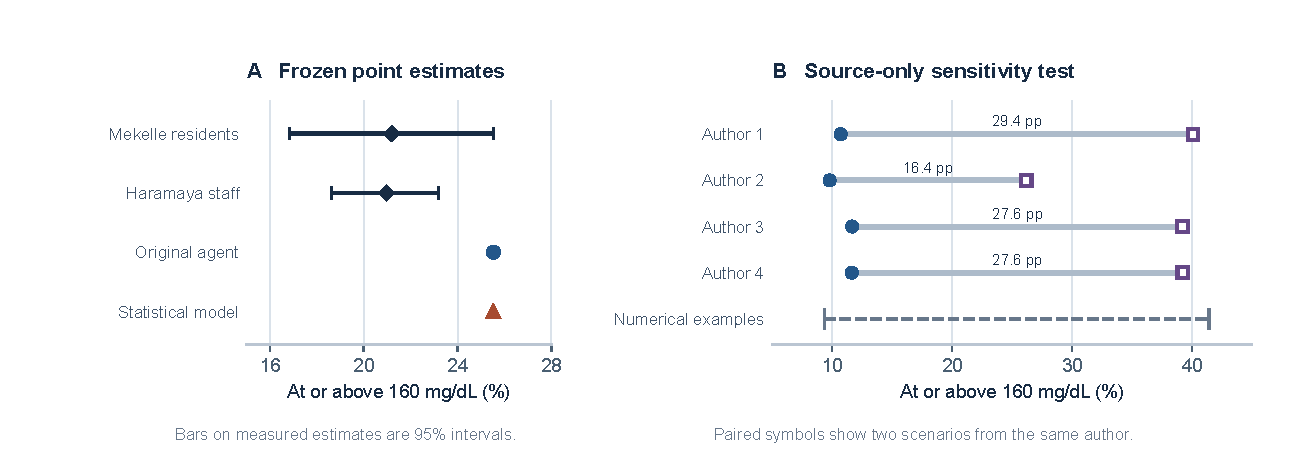
\includegraphics[width=.94\textwidth]{figures/nonhdl-selection.pdf}
\caption{What can a lipid screening study infer from the source? (A) A frozen agent and a statistical model independently selected similar joint laws. Diamonds and 95\% stratified bootstrap intervals summarize the two measured samples. (B) Four fresh authors received the same source summaries and were explicitly asked for two different, admissible joint models. Each line connects the pooled screening estimates for one author. The dashed segment joins two independently constructed numerical examples. The scenarios measure sensitivity at source.}
\Description{The original agent and comparator place about a quarter above the cutoff. In the separate experiment all four agents construct pairs of admissible models whose screening fractions differ by more than 16 percentage points.}
\label{fig:nonhdl}
\end{figure*}

\paragraph{Which use transferred?}
The common virtual mean was 128.77 mg/dL, compared with measured means of 125.12 in Mekelle and 123.58 in Haramaya. We did not assign a pass criterion to the mean. The primary threshold fraction was 25.53\% for the agent and 25.52\% for the statistical generator (Figure~\ref{fig:nonhdl}A). In Mekelle 68 of 321 participants reached the cutoff (21.18\%); in Haramaya 244 of 1,164 did (20.96\%). We had defined a study-planning tolerance of 20 additional people per 1,000. For the agent, the interval for the excess was $-0.02$ to 8.70 percentage points in Mekelle and 2.33 to 6.89 in Haramaya. The community result is unresolved under this rule. The employee result exceeds its upper limit. The statistical arm gave the same classifications. Both rates are sample estimates; the two recruitment frames afford separate checks within one country. The design compares transport of the complete laws. It cannot attribute the overestimate to pairing alone.

\paragraph{Can the agent construct the alternative?}
\begin{figure*}[t]
\centering
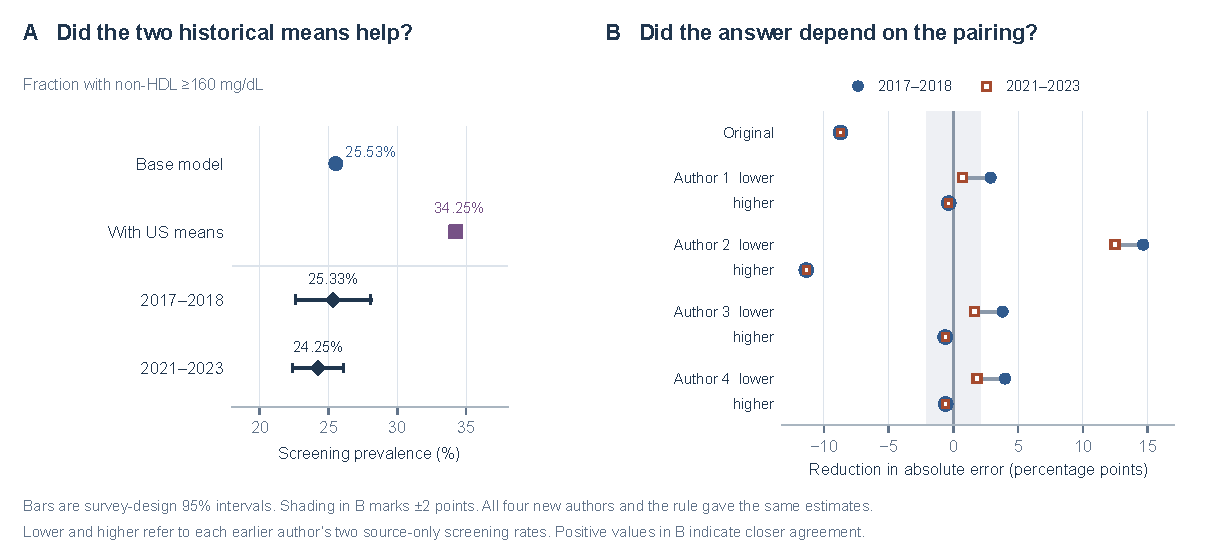
\includegraphics[width=.96\textwidth]{figures/historical-means-and-pairing.pdf}
\caption{Adding the same two historical US means to nine frozen lipid pairings. (A) On the original pairing the update raises the predicted screening rate above both later national estimates. (B) Each point shows the reduction in absolute error for one period and pairing. Positive values mean closer to the survey estimate. The line connects the two periods for a given pairing. Only panel A displays survey intervals. The four pairs of alternatives had been authored in a previous experiment.}
\Description{The original prediction goes from 25.53 to 34.25 percent. Both measured estimates are below 26 percent. For each of four authors, on both survey dates the alternative with the lower initial screening rate benefits at the survey point while the higher one deteriorates. Only one lower alternative benefits across both entire intervals.}
\label{fig:historicalmeans}
\end{figure*}

\begin{figure*}[t]
\centering
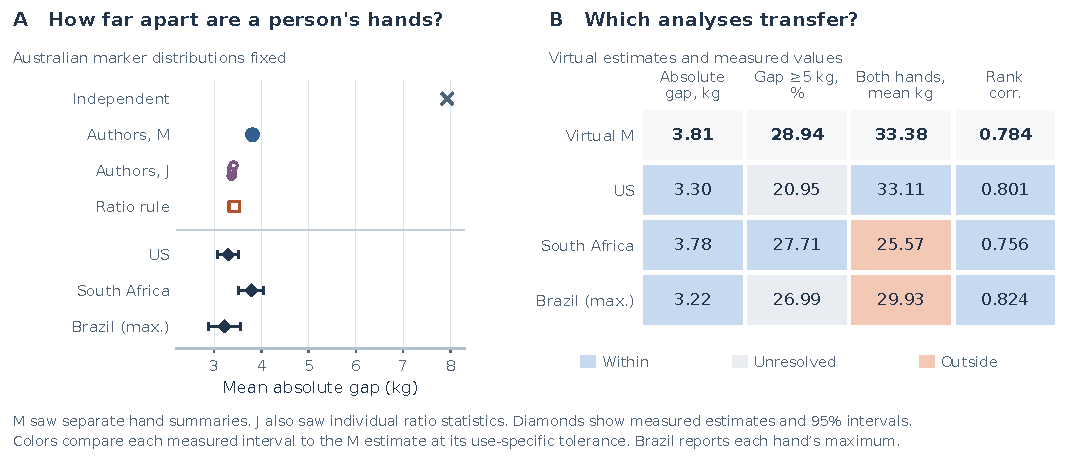
\includegraphics[width=.97\textwidth]{figures/bilateral-grip-transfer.pdf}
\caption{Pairing identical single-hand values changes the estimated difference between a person's hands. M authors saw separate Australian hand summaries. J authors also saw the dispersion of individual ratios in a German study. (A) Measured intervals cover sampling variation in each reference. (B) The same M table supports different analyses in different populations. The Brazil release uses each hand's maximum across attempts.}
\Description{Independent pairing gives a mean gap of 7.93 kg. The four M authors' common pairing gives 3.81, against 3.30 in the US and 3.78 in South Africa. A matrix compares four uses with complete sampling intervals. The South African and Brazilian bilateral means fall outside tolerance.}
\label{fig:grip}
\end{figure*}

Four fresh GPT sessions each wrote a program for two pairings using only the same source packet and fixed marginal values. They knew the requested analysis and saw neither the Ethiopian estimates nor the numerical comparator. We sealed all programs before execution, used three fixed seeds per scenario, and independently recomputed the checks. All 24 tables retained the exact marginal arrays, placed HDL at or below TC for every virtual person, and reproduced the reported mean individual ratio to within 0.00020. The non-HDL mean stayed at 128.77. Each author's two screening rates differed by 16.37--29.35 percentage points (Figure~\ref{fig:nonhdl}B). One calibrated opposite rank cycles to the same ratio. The other three used swaps guided by the screening threshold. A numerical assignment procedure found admissible examples at 9.38\% and 41.41\%. Their spread shows why the original agreement at 25.5\% supplies little evidence about which estimate to use. These deliberately different model pairs establish feasibility. Their frequency in a patient population remains unknown (Appendix~\ref{app:pairingtest}).

In a separate prospective study, eight advisers ranked six uses before opening a Virginia community sample. All groups prioritized mean non-HDL, which fell outside its tolerance. Seeing the alternative pairings moved the screening use to last place. Appendix~\ref{app:virginia} reports every decision and measured outcome.

\subsection{Do historical US means improve later US screening?}
Carroll et al.~\cite{carroll_history} reported mean TC of 196 mg/dL and HDL of 52.5 mg/dL in US adults in 2007--2010. Four fresh agents received these two means and the Mwanza evidence. Each could choose how much weight to give the US estimates and how to alter each marker's distribution while preserving ranks. All four chose proportional scaling to the two means, matching the statistical rule. We sealed their predictions under the original and all eight earlier alternative pairings before examining either later period.

Against 4,937 adults in 2017--2018 and 5,498 in August 2021--August 2023, the original virtual mean of individual TC/HDL ratios was 3.659. Both measured intervals lay within its prespecified $\pm0.30$ tolerance. This relationship was explicitly reported in Mwanza. For the primary analysis, non-HDL screening prevalence rose from 25.53\% to 34.25\%, increasing absolute error by 8.72 percentage points in both periods. Across the eight alternatives, the same marginal update brought four point predictions closer and moved four farther away in each period. Only one improvement held over both complete survey intervals. Figure~\ref{fig:historicalmeans} shows every pairing. Appendix~\ref{app:historicalmeans} reports all six uses and the survey design.



\section{Can the agent estimate how much a person's two hands differ?}
\label{sec:grip}
An Australian study reports the mean and SD of grip strength for each hand by age and sex~\cite{grip_adelaide}. How different are the two hands of one person? We fixed each hand's values within four sex-by-decade groups and asked four fresh agents to pair them. All four chose a Gaussian copula with correlation 0.80, producing the same permutation at every shared seed. The Australian table contained no such correlation.

We sealed the predictions before analyzing 1,423 US and 2,434 rural South African adults aged 50--69~\cite{grip_cdc,grip_haalsi}. Their measured mean absolute differences were 3.30 and 3.78 kg. The agents predicted 3.81 kg. Independent pairing of exactly the same values gave 7.93 kg. The agents reduced absolute error by at least 3.65 kg over both full reference intervals, exceeding the prespecified 1 kg improvement. Yet the same virtual records put South African mean grip strength 7.81 kg too high (Figure~\ref{fig:grip}).

Four further agents saw published German within-person ratio statistics~\cite{grip_ratio}. They predicted 3.37--3.41 kg, close to the statistical model's 3.42 kg using the same evidence. The added evidence improved the US point error but increased the South African one. Appendix~\ref{app:grip} gives the sampling uncertainty, a separate Brazilian measurement check, and the range compatible with the source summaries.



\section{Related work}
G-Sim uses an LLM to propose and revise simulators with numerical calibration~\cite{gsim}. LLMSynthor constructs micro-records aligned with macro statistics using discrepancy-guided generation~\cite{llmsynthor}. Filshtein et al.\ generate synthetic cohorts by sharing fitted models~\cite{filshtein}. SynthIPD reconstructs individual trial data from reports, and KMGen uses a skill-based agent for synthetic patient data from survival and adverse-event evidence~\cite{synthipd,kmgen}. SynthCraft supports healthcare data access and augmentation~\cite{synthcraft}. These works establish substantial prior art for both agentic simulation and generation from publications. Our experiments follow an agent's scientific choices into several estimands on the same output and compare each with an independently computed measured-sample analysis. The experiments supply a task-specific comparison of laws under identical information in Sections~\ref{sec:prospective} and~\ref{sec:ironpros}.

Statistical approaches can incorporate external summary information from heterogeneous populations~\cite{syndi}. The fact that moments leave other functionals partially identified has a long history, including distributional bounds with fixed margins and additional constraints~\cite{bounds,makarov,zaev}. Our prospective experiment uses an agent to construct and execute two examples and asks what this ambiguity means for a specific screening analysis. Work on inferential utility also shows that treating synthetic observations as measured records can understate uncertainty~\cite{inferential}. Here the virtual rows approximate the consequences of an assumed law. Model choice, source sampling variation and population transfer remain separate sources of uncertainty.

\section{Discussion}
A scientist can run the same analysis on several virtual cohorts, then ask which part of the answer the agent actually supplied. In Kenya the source group differences explained most of the adjusted BMI contrast. In CHNS, reassigning ferritin values within hemoglobin bands removed a contribution to the continuous correlation in every agent's original model. A better estimate for a single band nevertheless had little effect on whole-cohort accuracy. In Nigeria, six agents and a fitted statistical generator chose nearly the same dependence and substantially overestimated both measured associations. Numerical agreement across constructors can reflect a shared assumption. In handgrip, such an assumption improved the between-hand gap in two measured settings, while leaving a large error in the South African mean untouched.

The lipid experiments distinguish three uses of published evidence. Subtracting two means fixes mean non-HDL. The reported mean individual TC/HDL ratio carried over to two later national periods within its planning margin. Screening prevalence depended on the individual pairing. A uniform update to both marker distributions therefore helped some screening predictions and harmed others. Reporting an estimate alongside its dependence on these choices lets a researcher decide whether paired measurements would change the analysis.

The Brazilian pressure and US iron targets were exposed in development. The CHNS comparison used one within-survey split. Freetown's paired fields have an unresolved history, and the external Burkina Faso sample had no low-ferritin participant. Virginia supplied one community sample. The two later national periods share the historical source's survey family. Four lipid authors chose the same numerical update. Four grip authors chose the same pairing on the shared seeds. The two principal grip survey families had contributed other outcomes, and the Brazilian stress test used a different trial summary. These studies resolve particular scientific uses under stated evidence and tolerances. Transfer to a different recruitment frame requires its own measurements.

\bibliographystyle{ACM-Reference-Format}
\bibliography{references}
\appendix
\section{Construction, data and reproducibility}
\label{app:design}
\paragraph{Original papers.}
All six original-paper constructors used the requested and returned model identifier \texttt{gpt-6.1-sol}. Each had a fresh context and access to the task, the assigned article, supplementary search, the sampler contract and the generated-only inspection tool. The program, declared parameters and provenance notes were sealed before target comparison. The three final sampling seeds were 17121, 17123 and 17127. Each pressure draw had 3,000 rows and each iron draw 5,000. Estimators were also implemented independently using regression, counts and ranks. A target-family search preview in one pressure session contained survey identity, demographics and a qualitative topic. The session recorded and excluded it. The target slopes and paired correlation were withheld.

\paragraph{Pressure reference.}
The PNS operator uses the positive laboratory survey weight in a complete-case frame aged 20--79. It excludes recorded pregnancy. Unknown pregnancy status is retained under the frozen rule. The same rows enter both regressions. The design matrix contains an intercept, age, recorded sex and BMI in units of five kg/m$^2$. We correlate the residuals of the two pressure models. Synthetic records receive equal weights because the requested generator targets the weighted distribution. Five hundred row resamples retaining the survey weights gave conditional stability intervals of [2.96, 4.12] for the systolic slope, [1.93, 2.59] for the diastolic slope and [0.700, 0.734] for the residual correlation. The released workbook did not support a design-based cluster variance calculation.

\paragraph{Iron reference.}
NHANES August 2021--August 2023 supplies the measured hemoglobin, ferritin and survey-design variables. The eligible sample contains 979 nonpregnant women aged 20--44 with both measurements and positive phlebotomy weights. The frozen analysis uses raw ferritin with no inflammation adjustment. The three estimators are the weighted four-cell odds ratio, the weighted fraction with both markers low and a weighted Spearman correlation. A stratified delete-one-primary-sampling-unit calculation with 15 strata and 30 primary sampling units gave 95\% intervals of [9.28, 34.11] for the odds ratio, [6.07, 9.55]\% for both markers low and [0.318, 0.473] for the rank correlation.

\paragraph{Controlled evidence.}
The pressure and iron controls used nine fresh constructors each, with three seeded draws per constructor. The source block was masked before the modeling call. For pressure this hid or revealed six same-sample entries relating SBP, DBP, BMI and age. For iron it hid or revealed a paired contingency table. Neither experiment supplied the desired target result. The common base differed between cases, so cross-case comparisons of the base arm do not measure a shared zero-information condition. Both experiments used one model call per constructor, no feedback round and the same GPT identifier as the original-paper trials. Usage valued at the recorded tariffs was US\$0.92 for pressure and US\$0.68 for iron.

\paragraph{What orchestration adds.}
A separate developmental comparison started both an ordinary coding agent and a structured workflow from a research request. They had the same GPT model, search and runtime capabilities, and resource limits. Across 12 constructions and 36 seeded tables, the ordinary agent had smaller mean absolute discrepancies on four of the six focal analyses and the structured workflow on two. This result supports using a simple agent as a viable constructor. The source-to-code records serve the separate purpose of making each scientific choice inspectable.

\paragraph{Use of generative AI.}
The construction experiments used the model recorded above. OpenAI Codex also assisted in drafting the English manuscript, preparing the \LaTeX{} files and checking reported numerical results against the experimental artifacts.

\section{CHNS holdout, paired evaluation and local decomposition}
\label{app:chns}
\begin{figure*}[t]
\centering
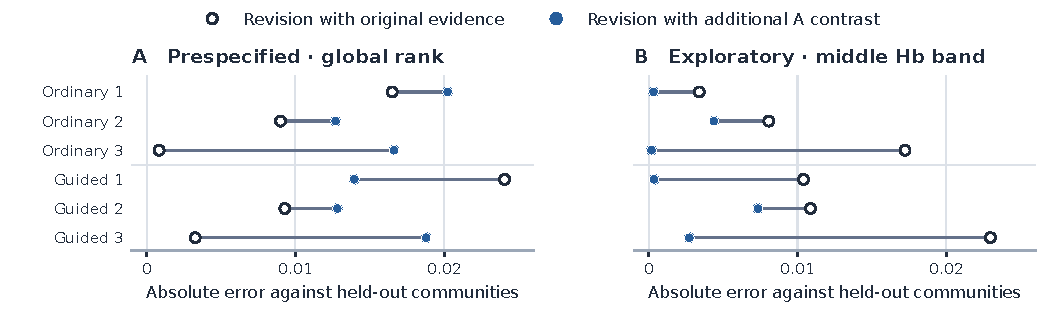
\includegraphics[width=.98\textwidth]{figures/chns-revision.pdf}
\caption{What changed when a constructor received one extra conditional contrast? Each row pairs two revisions of the same parent. Leftward movement means smaller absolute error against CHNS B. (A) On the prespecified whole-cohort rank correlation, one of six moves closer. (B) In a post hoc decomposition, all six move closer on the middle Hb band's weighted contribution to the global correlation. The two panels use the same scale. The B reference is a sample estimate.}
\Description{Paired error plots for three ordinary and three workflow constructors. Additional evidence lowers whole-cohort rank error for the first workflow constructor. It reduces the error in the middle-band contribution for every constructor.}
\label{fig:revision}
\end{figure*}
\paragraph{Population.}
We linked 2,218 age-eligible women with the required survey fields. Of these, 2,205 had positive paired measurements. We converted the central Hb field from g/L to g/dL. Serum ferritin in ng/mL is numerically equal to $\mu$g/L. Ferritin was uncorrected for inflammation. Eligibility included all recorded pregnancy and inflammation statuses. We analyzed complete cases without national survey weights. Estimates describe this sample of women. Within province, a fixed hash ordering assigned alternate communities to A and B. We sealed the split, input hashes, research questions, tolerances and evidence schedule before model calls. The study articles supplied no measurements from B.

\paragraph{Construction.}
Each arm had three initial sessions. We interleaved the sessions and used the same GPT configuration and isolated runtime throughout. Each of the six parent programs had two sealed sibling revisions. One saw the original evidence and the source checks on the parent. The other also saw the added A contrast. All 18 requests returned programs. Each program drew 12,000 records at each of three common seeds. The scientific analysis pooled the three draws per program. The 54 tables are simulation repeats nested within six parents and one survey split. The 18 calls cost US\$1.77 at recorded token tariffs. A separate implementation reproduced the table analyses, the B intervals and both arm decisions before manuscript integration.

We computed Spearman correlation from average ranks for ties. For the crude odds ratio B had 114 both markers low, 116 only Hb low, 161 only ferritin low and 691 neither. The odds ratio is $(114\times691)/(116\times161)=4.218$. All four cells exceeded the minimum of ten. We used 2,000 province-stratified whole-community bootstrap replicates in each half. The B interval for correlation met the prespecified precision rule (half-width at most 0.10). The study's final-use rule required absolute rank error at most 0.10, an augmented odds ratio within a factor of 1.50 of B's, and augmented and control odds ratios within a factor of 1.20 of one another. All six passed. The primary incremental contrast subtracts augmented absolute rank error from control absolute rank error. A material arm-level benefit required all three pairs, median gain at least 0.05 with lower bootstrap limit above zero, at least two final-use passes and sufficient B precision. Conditional on the three parents per arm, the 95\% B-sampling intervals for the median gains were [$-0.0037$, $0.0037$] and [$-0.0035$, $0.0090$] for ordinary and guided sessions, respectively. Neither arm met the rule.

\begin{table*}[t]
\caption{All six CHNS sibling comparisons, with three pooled draws per program. C denotes revision with the original evidence. E denotes its sibling given the additional A contrast. A positive gain is a reduction in absolute error for the whole-cohort correlation. The final two columns describe errors in the probability-weighted middle-band contribution, examined after B was opened.}
\label{tab:chns}
\centering
\begin{tabular}{@{}lrrrrrr@{}}
\toprule
 & \multicolumn{4}{c}{Prespecified whole-cohort analyses} & \multicolumn{2}{c}{Exploratory local error}\\
\cmidrule(lr){2-5}\cmidrule(l){6-7}
Parent & Rank C & Rank E & Rank gain & Odds ratio E & C & E\\
\midrule
Ordinary 1 & 0.3003 & 0.2966 & $-0.0037$ & 5.1149 & 0.0034 & 0.0003\\
Ordinary 2 & 0.3078 & 0.3041 & $-0.0037$ & 4.9900 & 0.0081 & 0.0044\\
Ordinary 3 & 0.3176 & 0.3002 & $-0.0158$ & 5.1224 & 0.0172 & 0.0002\\
Guided 1 & 0.2927 & 0.3028 & $+0.0101$ & 5.0992 & 0.0104 & 0.0004\\
Guided 2 & 0.3075 & 0.3040 & $-0.0035$ & 5.1237 & 0.0109 & 0.0073\\
Guided 3 & 0.3201 & 0.2980 & $-0.0155$ & 4.9924 & 0.0230 & 0.0027\\
\bottomrule
\end{tabular}
\end{table*}

\paragraph{Exploratory covariance partition.}
Let $U,V$ denote global sample midranks of Hb and ferritin, each centered and standardized to unit variance with the full sample denominator. Let $G$ partition Hb at 12 and 14 g/dL. Then
\begin{align*}
\rho_S
  &= \operatorname{Cov}\{\mathbb E[U\mid G],\mathbb E[V\mid G]\}\\
  &\quad +\sum_g \Pr(G=g)\operatorname{Cov}(U,V\mid G=g).
\end{align*}
The middle-band value uses the original global ranks with the band-specific covariance and the band's sample weight. Reranking participants within the middle band would define a different statistic. In B, the between-band term was 0.270538 and the within-band terms were 0.011512, 0.034290 and 0.000460. Their sum gives 0.316800 up to rounding. For Guided 3 the middle contribution changed from 0.05726 to 0.03702 while the global rank correlation moved farther from B. Across parents, the between-band estimates were 0.2444--0.2489 with the original evidence and 0.2444--0.2474 with the extra contrast. Table~\ref{tab:chns} retains both the predeclared endpoints and the six descriptive component comparisons.

\begin{table*}[t]
\caption{What did the CHNS A evidence alone supply? The B reference is a Spearman correlation of 0.3168 and a crude odds ratio of 4.218. All four rows use only the original evidence. The retrospective statistical model and each of the six agent models use 36,000 draws per law. Ranges cover the six original-evidence agents. Re-pairing gives the expected correlation under a uniform permutation within each Hb band and leaves each agent's four threshold counts unchanged.}
\label{tab:chnsattribution}
\centering
\begin{tabular}{@{}lrrrr@{}}
\toprule
 & \multicolumn{2}{c}{Continuous Hb and ferritin} & \multicolumn{2}{c}{Threshold association}\\
\cmidrule(lr){2-3}\cmidrule(l){4-5}
Construction & Spearman $\rho$ & $|\rho-\rho_B|$ & Odds ratio & $|\log(\mathrm{OR}/\mathrm{OR}_B)|$\\
\midrule
Direct A threshold counts & --- & --- & 5.083 & 0.187\\
Statistical model, independent within Hb band & 0.2370 & 0.0798 & 5.023 & 0.175\\
Agent records, expected after within-band re-pairing & 0.2444--0.2489 & 0.0679--0.0724 & 4.998--5.175 & 0.170--0.205\\
Agent records, original pairing & 0.2927--0.3201 & 0.0008--0.0241 & 4.998--5.175 & 0.170--0.205\\
\bottomrule
\end{tabular}
\end{table*}

\paragraph{Incremental effect on the prespecified whole-cohort analysis.}
The revisions using only the original evidence reproduced all 18 initial tables byte for byte at the three shared seeds. Five of six augmented laws came closer to the supplied A contrast on the log scale. In B only one came closer on whole-cohort rank correlation (Figure~\ref{fig:revision}A). Median reductions in absolute rank error were $-0.0037$ for ordinary and $-0.0035$ for guided constructors. The prespecified material gain was 0.05. The largest control error against B was 0.024, already below that benchmark. Even a perfect revision at the observed B estimate could therefore have gained at most 0.024.

For the middle-band within-group contribution, median absolute error fell from 0.01064 to 0.00155. Errors in this component and the between-band component could offset one another. Table~\ref{tab:chns} gives the individual comparisons.

\subsection{A statistical model using the original CHNS evidence}
\label{app:chnsstat}
The retrospective comparator uses the same evidentiary inputs as the six original-evidence parents. The Zhu article supplies the scientific context and definitions. The A tables give numerical constraints in the survey population, so we use their counts and moments wherever the sources overlap. The model was specified after B was public. We recorded its equations, source hierarchy, scoring code, seeds and input hashes before scoring its draws. This compares statistical constructions given extracted evidence. It does not test article retrieval or extraction.

Let $G$ denote the three Hb bands. The model samples $G$ with probability $n_g/1123$. Conditional on $G$, it samples Hb and ferritin independently. For Hb we fit a beta distribution by moments on $(0,12)$ or $(12,14)$ and a shifted gamma law above 14. For $Y=\log(\mathrm{ferritin})$ we use the maximum-entropy density subject to the reported log mean, log variance and probability below $k=\log 15$. It has the form
\[
q_g(y)\ \propto\ \exp\{a_g y+b_g y^2+c_g\,\mathbf{1}_{y<k}\},\qquad b_g<0 .
\]
This is a normal density reweighted on either side of $k$. We set the two masses using the reported depletion frequency and solve for the underlying normal location and scale by matching the two log moments. At the resulting solution, every competing density satisfying the constraints has the same expectation of $\log q_g$. Nonnegativity of relative entropy then gives the stated entropy maximum on the log scale. This is one choice of marginal family and one assumption about dependence. Numerical integration verified all three fitted probabilities, means and dispersions against the A tables.

For the analytic population rank let $w_g=\Pr(G=g)$, $u_g=\sum_{j<g}w_j+w_g/2$, and $F_Y$ be the mixture CDF of log ferritin. Since the Hb bands are ordered and the two markers are independent within a band, $\rho_S=12\sum_g w_g u_g \mathbb E[F_Y(Y)\mid G=g]-3$. Integration gives 0.2414 and the four source cells give an OR of 5.083. The three 12,000-row draws gave ranks of 0.2456, 0.2451 and 0.2198. Pooling the records with the original estimator gives Table~\ref{tab:chnsattribution}. Direct per-draw rank and cell calculations reproduced both endpoints. The comparison uses zero additional model calls.

The re-pairing row uses the existing agent records. Under a random permutation of ferritin within each Hb band, the expected within-band covariance of the standardized global midranks is zero. All ranks and the number of threshold crossings per band retain their original marginal values. The between-band covariance in the preceding decomposition is therefore the exact expected Spearman correlation under that permutation. Table~\ref{tab:chnsattribution} reports its distance from B's estimate. The paired absolute-error reductions from the authored pairing ranged from 0.0454 to 0.0713. This is a conditional comparison on the six saved laws; the three seeds per law approximate that law's output.

\section{Every original-paper outcome}
\label{app:profiles}
\begin{figure*}[t]
\centering
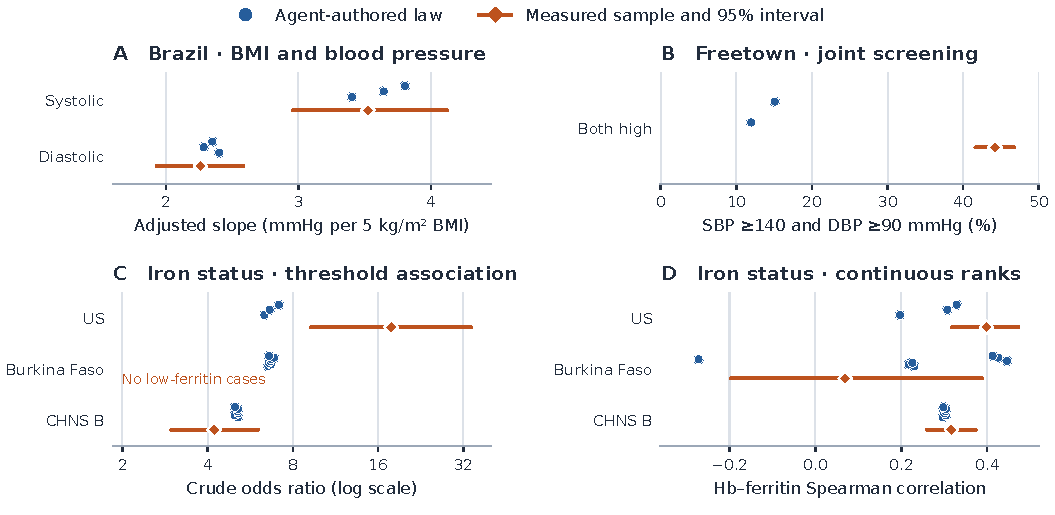
\includegraphics[width=.98\textwidth]{figures/analysis-support.pdf}
\caption{What the virtual cohorts support when the scientific analysis stays fixed. Each circle is one agent-authored law. Diamonds and bars show measured estimates and their 95\% intervals. (A) Three constructors recover the scale of the adjusted Brazilian blood-pressure slopes. (B) Two laws that share five source moments both understate the joint screening rate in the deposited Freetown fields. (C, D) Each iron cohort supplies both a threshold odds ratio and a continuous rank correlation. Burkina Faso has no low-ferritin cases. In CHNS the six final laws meet both prespecified planning tolerances. Brazil and the US are development comparisons. Freetown and Burkina Faso are external assessments. CHNS B comprises communities held out within a survey. The Brazilian bars describe row-resampling stability.}
\Description{Four panels compare modeled and measured quantities in their native units. Blood-pressure slopes are close in Brazil. The Freetown joint rate is much higher in the release. Iron models preserve the source odds ratio in the US and Burkina Faso tasks while continuous ranks vary. Both CHNS analyses show positive associations near the held-out estimates.}
\label{fig:support}
\end{figure*}

\begin{figure*}[t]
\centering
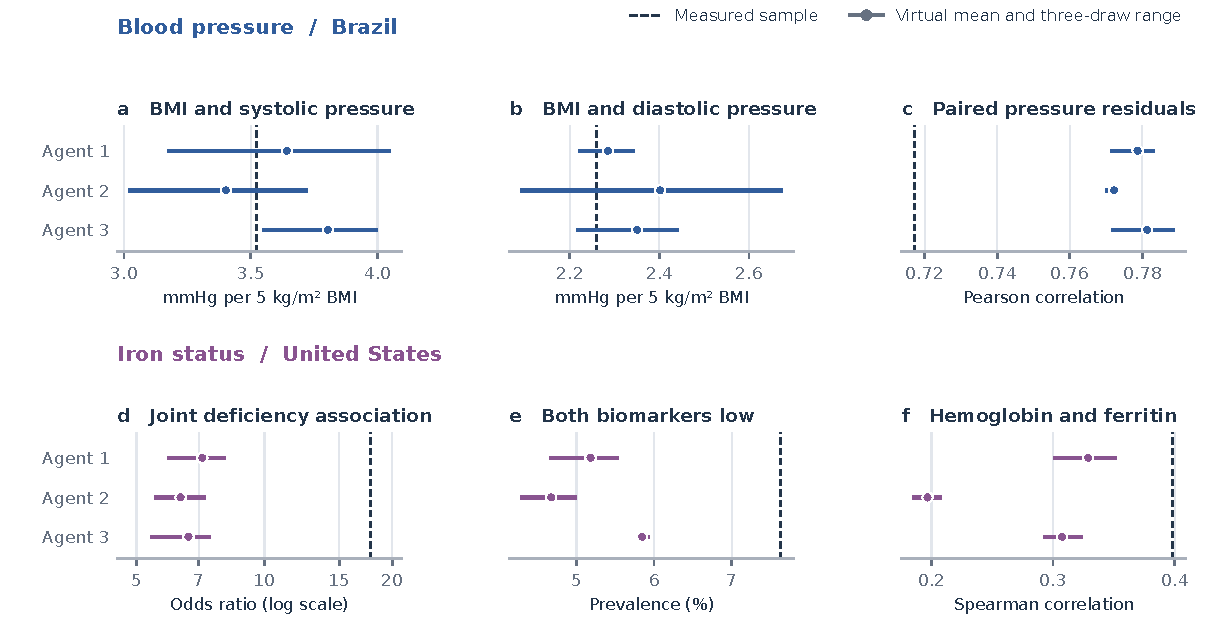
\includegraphics[width=.85\textwidth]{figures/original-paper.pdf}
\caption{The same analysis run on virtual and measured records. Each point is one constructor's mean across three seeded draws. The segment spans those draws. Dashed lines are measured sample estimates. Each panel has its own scale. The systolic slopes are near the Brazilian estimate. The iron odds ratios cluster around the value derived from the Chinese source paper, well below the US estimate.}
\Description{Six panels compare three constructors with a measured reference. The three systolic slopes straddle the reference, all diastolic slopes and residual correlations exceed it, and all three iron odds ratios, joint prevalences and rank correlations fall below their reference.}
\label{fig:original}
\end{figure*}

Table~\ref{tab:profile} preserves all three primary endpoints and the accompanying diagnostics in each case. Author numbers identify independent sessions within one task. The zero ordering violation rate follows from the positive pulse-pressure construction. Across the iron sessions, the two marginal deficiency fractions move in opposite directions relative to the US sample. The isolated threshold odds ratio is therefore an incomplete guide to biomedical utility.

\begin{table}[htbp]
\caption{All original-paper estimates. A1--A3 are constructor means over three seeded draws. The final column is the measured sample. Percentages use a 0--100 scale.}
\label{tab:profile}
\centering
\begin{tabular}{@{}lrrrr@{}}
\toprule
Analysis & A1 & A2 & A3 & Measured\\
\midrule
\multicolumn{5}{@{}l}{\emph{Brazilian blood pressure}}\\
BMI--SBP slope & 3.642 & 3.402 & 3.804 & 3.524\\
BMI--DBP slope & 2.285 & 2.402 & 2.350 & 2.260\\
Residual correlation & .779 & .772 & .781 & .717\\
SBP SD (mmHg) & 20.00 & 19.70 & 19.57 & 18.19\\
DBP SD (mmHg) & 11.57 & 11.57 & 11.47 & 11.09\\
SBP $<$ DBP (\%) & 0 & 0 & 0 & 0\\
\midrule
\multicolumn{5}{@{}l}{\emph{US iron status}}\\
Threshold odds ratio & 7.141 & 6.348 & 6.625 & 17.790\\
Both low (\%) & 5.180 & 4.673 & 5.847 & 7.630\\
Spearman correlation & .329 & .197 & .307 & .398\\
Low hemoglobin (\%) & 10.660 & 8.807 & 11.727 & 15.240\\
Low ferritin (\%) & 15.680 & 18.513 & 17.487 & 12.153\\
\bottomrule
\end{tabular}
\end{table}

\section{Two blood-pressure laws under the same constraints}
\label{app:freetownaccount}
\label{app:laws}

\begin{figure*}[t]
\centering
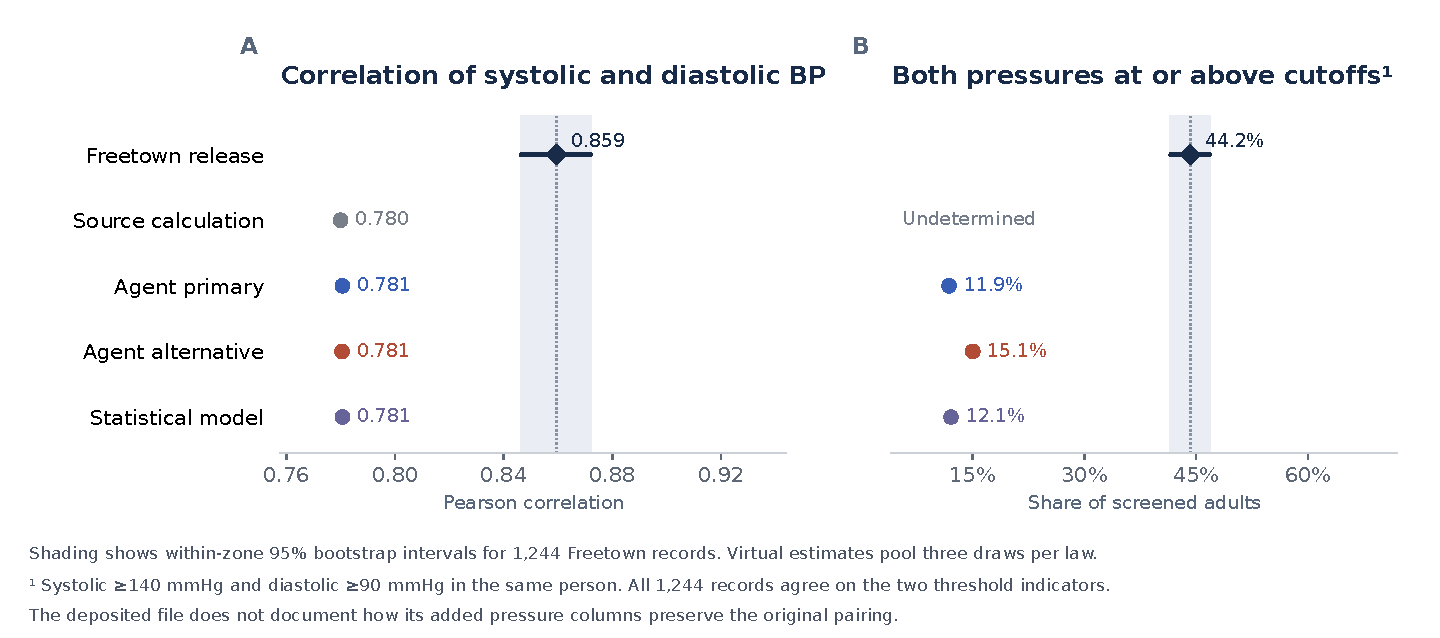
\includegraphics[width=.84\textwidth]{figures/freetown.pdf}
\caption{Prospective screening test. The source correlation is available by direct calculation. The joint threshold probability depends on the model. Points for the two agent laws and the statistical comparator are estimates from seeded virtual draws. The band describes uncertainty for the deposited Freetown sample conditional on the represented zones. The extreme target threshold result led to a separate audit of the deposited fields.}
\Description{Two panels show a released correlation of 0.859 and a joint threshold percentage of 44.2. Three virtual arms give correlations near 0.78 and threshold percentages between 11.9 and 15.1.}
\label{fig:freetown}
\end{figure*}

Let $S$ and $D$ be systolic and diastolic pressure. Write $G=S-D$ for the pulse-pressure gap. From the five source statistics, calculate
\begin{align*}
\mathrm{E}[G] &= \mathrm{E}[S]-\mathrm{E}[D],\\
\mathrm{Cov}(D,G) &= \mathrm{Cov}(S,D)-\mathrm{Var}(D),\\
\mathrm{Var}(G) &= \mathrm{Var}(S)+\mathrm{Var}(D)-2\mathrm{Cov}(S,D).
\end{align*}
The primary program draws positive $(D,G)$ from a bivariate lognormal distribution with these moments. For a vector of positive means $m$ and covariance $V$, the log covariance entries are $\log(1+V_{ij}/(m_i m_j))$ and the log means are $\log m_i$ minus half the corresponding log variance. Here the resulting matrices are positive definite. Setting $S=D+G$ enforces the intended ordering in every row.

The alternative program assigns probabilities 0.75 and 0.25 to components with means $(S,D)=(116.22,76.54)$ and $(152.22,92.54)$ mmHg. In $(D,G)$ coordinates, each component receives a common within-component covariance equal to the required total covariance minus the covariance of the component means. By the total covariance identity this gives the same unconditional first and second moments. The component probabilities and offsets are modeling choices. Conditional-normal quadrature for the event $\{D\geq90,\ D+G\geq140\}$ gives the probabilities in Section~\ref{sec:prospective}. Moments alone do not select either law.

\paragraph{Pre-disclosure design and measurement.}
The team screened eligibility, headers, uniqueness, measurement methods and field completeness before fixing the Freetown analysis. The target release identity and outcomes were withheld from the constructor. The primary, alternative, comparator, judgments and integration results were recorded before inspecting the measured joint outcomes. Construction took one recorded GPT call (US\$0.0845 at the recorded tariff). Each law generated three equal-sized draws of 10,000, including three for the independently implemented statistical comparator. The source protocol averaged the last two of three seated readings after at least 15 minutes' rest. Freetown averaged two readings following 3--5 minutes of rest. The source selected partnered rural adults, whereas the target was an urban community screening sample.

The Freetown reference uses paired positive recorded pressure values in prespecified age categories covering adults 40 and older. We computed an unweighted sample correlation and exceedance fraction. Intervals use 2,000 bootstraps of participants within eight zones, conditional on those zones. Across the full release, the audit counted 871 records meeting both thresholds, 1,523 meeting neither and zero in either discordant cell. These counts refer to deposited values. Field-level provenance would be needed to explain the pattern.



\subsection{The prospective Freetown comparison}
Before inspecting paired outcome values in a new Freetown screening release~\cite{freetown,freetowndata}, we specified two analyses: the unadjusted Pearson correlation of SBP and DBP, and the fraction simultaneously reaching 140 mmHg systolic \emph{and} 90 mmHg diastolic. The latter is a conjunction of two thresholds. It has a different interpretation from a clinical hypertension diagnosis. The agent received five rounded source summaries from the rural Burkina Faso study~\cite{jaspert}, comprising means 125.22 and 80.54 mmHg, standard deviations 18.22 and 10.98 mmHg, and raw correlation 0.78. It also received the target sampling context. This experiment starts from extracted summaries. The earlier experiments in Section~\ref{sec:original} test original-paper reading.


One fresh agent was asked to propose a primary and an alternative law and state which analyses the source constrained. Before disclosure, it identified the correlation as reported, the joint threshold as underdetermined and the application to a new population as uncertain. Its primary model coupled positive DBP and pulse pressure with a bivariate lognormal law. A statistical comparator specified in advance from the same five numbers independently used this family. The agent's alternative was a 75:25 mixture. It separated the component means and subtracted their between-component contribution from the within-component covariance. These are hypothetical population structures. Both laws preserve all five working moments, including an exact population correlation of 0.780.

Independent numerical integration of the fixed programs gave joint threshold probabilities of 11.9449\% and 15.0851\%. These two examples establish a 3.14 percentage-point difference consistent with the five summaries. They give a lower bound on the range of answers permitted by those constraints. The full range may be wider. A separately prespecified finite-draw criterion asked whether the simulated gap, after subtracting four times the sum of Monte Carlo standard errors, exceeded two percentage points. The adjusted gap was 1.60 points, below the criterion. We report both results because they answer different questions.

After the freeze we analyzed the deposited fields of 1,244 eligible screening participants aged 40 or older. Their correlation was 0.859 (within-zone bootstrap 95\% interval 0.847--0.872), and 44.21\% met both thresholds (41.64--46.79\%). All three simulated arms were far below the released joint rate (Figure~\ref{fig:support}B and Appendix Figure~\ref{fig:freetown}). A post-disclosure count clarified how to interpret that difference. Of the eligible records, 550 met both thresholds, 694 met neither, and neither isolated exceedance occurred. The same pattern held across all 2,394 released records. The codebook identifies the component fields as added variables. Their pairing history remains unresolved. The measured discrepancy applies to the deposited fields. The unresolved pairing limits its biological interpretation.

\section{Original-paper iron construction and verification}
\label{app:ironpros}

\begin{figure*}[t]
\centering
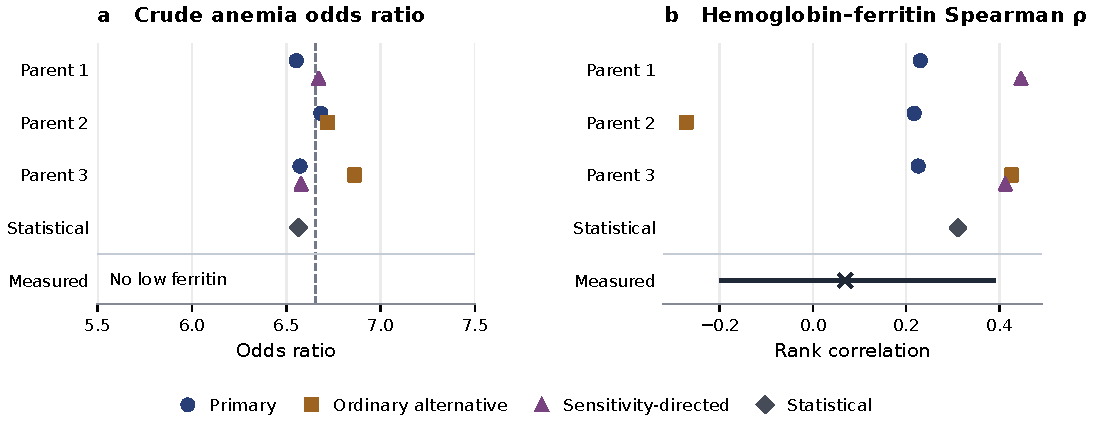
\includegraphics[width=.98\textwidth]{figures/iron-alternatives.pdf}
\caption{Two analyses on each sealed iron cohort. Symbols in each parent row distinguish the primary law and the two alternative requests. Two requests reached the output limit and have no point. The dashed line marks the source odds ratio of 6.65. The measured row gives the survey-weighted result for 44 women. The rank interval resamples villages within province. No woman in this sample had low measured ferritin.}
\Description{Agent odds ratios cluster between 6.55 and 6.86. Their rank correlations range from minus 0.272 to plus 0.446. The measured rank correlation is 0.069, with a wide interval.}
\label{fig:ironpros}
\end{figure*}

The protocol specified three independent primary sessions, two branches per primary, three seeds per executable law and 20,000 independent draws per seed. GPT-6.1 Sol received the original paper and a target description. It supplied the structure, parameters, prospective judgments and Python code. The statistical comparator used the same source and independent within-cell ranks. Two of nine requests (ordinary branch of parent 1, directed branch of parent 2) exhausted the 12,288-token output allowance. Usage across all nine requests cost an estimated US\$1.37 at the recorded tariff.

The original interface failed on all seven complete programs. Each program expected its named parameters at a different nesting level than the runner supplied. After the primary submissions were inspected and before simulated or measured outcomes were examined, we registered one mechanical rule to pass the nested parameter object following the same missing-key error on all three seeds. This rule preserved every scientific constant, line of sampler code, seed and target task. Original executions, failures and corrected executions were archived separately. The seven agent programs and one statistical program then produced 24 tables. All source assessments and model comparisons were committed before external disclosure.

The source checks cover four crude-cell frequencies, the crude log odds ratio, three hemoglobin-band frequencies, three ferritin-depletion fractions, three within-band ferritin geometric means, and both overall geometric means. These 16 checks overlap. Tolerances allow rounding, four estimated Monte Carlo standard errors and fixed operational allowances. Table~\ref{tab:ironprospective} gives the pooled simulated estimates. Each completed pair's absolute rank gap was 0.187--0.489. Subtracting its estimated 95\% Monte Carlo margin left 0.175--0.475. These margins describe simulation precision conditional on fixed laws.

\begin{table}[H]
\caption{Prospective iron analyses by parent and request. Each completed law contributes three draws. The last column records the complete source screen.}
\label{tab:ironprospective}
\centering
\begin{tabular}{@{}lrrl@{}}
\toprule
Construction & Odds ratio & Spearman $\rho$ & Screen\\
\midrule
P1 primary & 6.553 & 0.230 & pass\\
P1 ordinary & -- & -- & incomplete\\
P1 directed & 6.672 & 0.446 & pass\\
P2 primary & 6.683 & 0.217 & pass\\
P2 ordinary & 6.718 & -0.272 & pass\\
P2 directed & -- & -- & incomplete\\
P3 primary & 6.573 & 0.226 & pass\\
P3 ordinary & 6.862 & 0.426 & pass\\
P3 directed & 6.579 & 0.413 & pass\\
Statistical & 6.564 & 0.311 & pass\\
\bottomrule
\end{tabular}
\end{table}

\paragraph{What choices changed the continuous association?}
Three primary authors each received the article and the research request. Follow-up authors received a sealed primary program and either a request for another defensible model or for a sensitivity model. Four of the six requested pairs completed. In all four, the change in rank exceeded its simulation noise. Only one primary yielded both alternatives. For the second parent, the ordinary alternative used a Gaussian copula parameter of $-0.75$ within bands and changed rank correlation from $0.217$ to $-0.272$. This was an explicit assumption. For the third parent the two positive-dependence alternatives moved its rank from $0.226$ to $0.426$ and $0.413$. The 44 measured mothers came from 23 villages. Eighteen had low hemoglobin, none had low ferritin, and both binary classifications agreed with the deposited flags for every woman.

\section{What can change while the selected iron summaries stay fixed?}
\label{app:ironproof}
Consider a single published hemoglobin band and ferritin-depletion cell with positive probability. Keep its probability and the two continuous conditional marginal distributions fixed. Draw hemoglobin from its conditional quantile function at a uniform rank $U$. One law draws ferritin from its conditional quantile at an independent uniform rank $V$. Another draws ferritin at $U$ with probability $\lambda>0$ and at $V$ otherwise. All other cells can stay fixed. The four threshold counts, each hemoglobin-band probability, and the ferritin geometric mean and depletion frequency in each band are invariant in the population. The overall geometric means are invariant as well.
For continuous marginal distributions, Spearman correlation is $12\,\mathbb{E}[F_H(H)F_F(F)]-3$. Within a nondegenerate cell the two marginal ranks are increasing functions of their corresponding uniforms. Sharing a uniform gives them positive covariance relative to independence. Hence the overall rank correlation changes while all the listed summaries remain fixed. This construction explains the ambiguity for the specified summaries. It supplies neither a biological estimate of the coupling nor its feasible range under additional evidence.

\section{Matched-size lifestyle analysis}
\label{app:lifestyle}

\begin{figure*}[t]
\centering
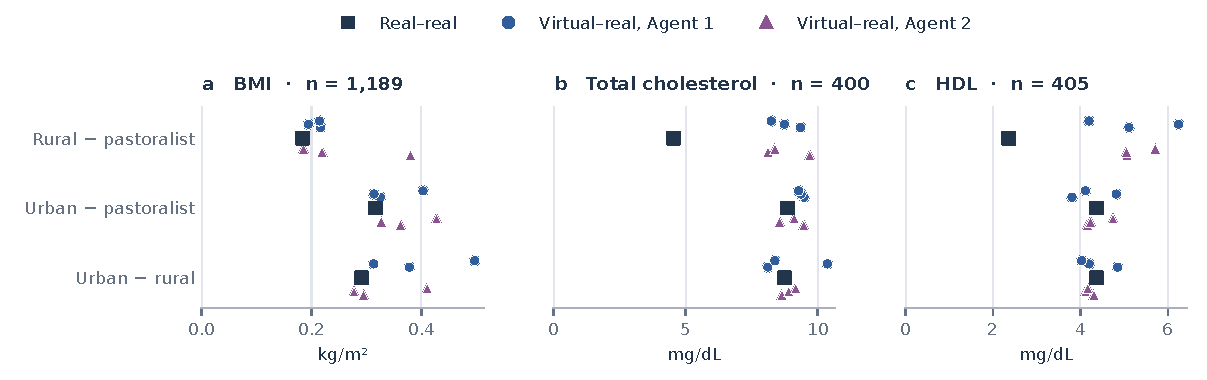
\includegraphics[width=.92\textwidth]{figures/lifestyle.pdf}
\caption{Matched-size mean absolute discrepancies for all nine adjusted lifestyle contrasts. The real--real estimate comes from two resamples of measured records. The virtual--real estimates use six saved virtual tables from two constructors. Native units and sample sizes differ across panels.}
\Description{Three panels compare BMI, total cholesterol and HDL across rural, urban and pastoralist lifestyles. Virtual versus real discrepancies are similar to real versus real for the urban BMI contrast, and larger for both rural lipid contrasts.}
\label{fig:lifestyle}
\end{figure*}

The original Turkana regression compared three lifestyle groups, adjusting each trait for age and sex~\cite{lea}. Real and virtual samples were matched on six sex-by-lifestyle stratum sizes within each trait. There were 1,189 eligible BMI measurements, 400 total cholesterol measurements and 405 HDL measurements. Each of 500 repetitions drew two real samples from the same empirical pool and one sample from each fixed virtual table. The virtual samples shared the second real sample as their reference. This design conditions on sample size, available cases and stratum counts. It leaves age and the outcomes free to vary. The bootstrap uses participants and does not model household or site clustering.



\begin{table*}[t]
\caption{Absolute discrepancies in matched-size lifestyle regressions. R and U denote rural and urban groups, and P denotes pastoralists. V--R gives the range across six fixed tables.}
\label{tab:lifestyle}
\centering
\begin{tabular}{@{}llrr@{}}
\toprule
Outcome & Contrast & Real--real & V--R\\
\midrule
BMI & R--P & .184 & .185--.380\\
(kg/m$^2$) & U--P & .316 & .314--.428\\
 & U--R & .291 & .277--.497\\
\midrule
Total cholesterol & R--P & 4.543 & 8.118--9.695\\
(mg/dL) & U--P & 8.848 & 8.556--9.479\\
 & U--R & 8.743 & 8.110--10.365\\
\midrule
HDL cholesterol & R--P & 2.363 & 4.195--6.242\\
(mg/dL) & U--P & 4.375 & 3.807--4.818\\
 & U--R & 4.362 & 4.029--4.851\\
\bottomrule
\end{tabular}
\end{table*}

Only 37 urban participants contributed total cholesterol measurements and 38 contributed HDL measurements. This small group helps explain the wide real--real variation. The discrepancy estimates in Table~\ref{tab:lifestyle} describe the observed composition. Equivalence for a planning decision would require a tolerance justified for that decision.

\section{Prospective external comparison in Akwa Ibom}
\label{app:akwa}
The Akwa Ibom study in southern Nigeria was second on the project's previously ordered list of iron cohorts. We screened the data dictionary, release terms, availability and uniqueness of participant keys before measuring either endpoint. Among the 1,290 biochemical records, 603 female participants in the mothers' group were aged 18--49 and had positive, finite Hb and serum ferritin. They came from 30 enumeration areas in 10 local government areas. The biochemical file supplies no analysis weight or pregnancy indicator. We report the sampled mothers' crude rank correlation and threshold odds using uncorrected ferritin. These characteristics limit transport from the Chinese cohorts. IITA and HarvestPlus supervised the original survey with support from the Bill \& Melinda Gates Foundation to HarvestPlus~\cite{akwa_iron}.

The article, aggregate supplement, task, seeds and hidden data digest were fixed before dispatch. The common virtual marginals came from the source-only CHNS A fit. Every law received the same sorted Hb and ferritin values in each of three Hb bands. The agent returned a sampler that assigns a permutation of ferritin values to the Hb values in each band, plus its parameters and their rationale. Six fresh sessions used the same GPT configuration. For the statistical arm we fit one Gaussian copula parameter to the supplied geometric-mean ferritin ratio of 1.215 comparing $13\leq\mathrm{Hb}<14$ with $12\leq\mathrm{Hb}<13$. Numerical integration gave a latent normal correlation of 0.137. The statistical law used this value in all three bands. Each law received the same three seeds and 12,000 virtual pairs per seed. Pairing preserves the threshold counts exactly across arms. The source ratio and each law's realized middle-band contrast remain available for checking.

We pooled each law's three draws for scoring and resampled whole enumeration areas within each local government area 2,000 times. Each paired bootstrap replicate compared all frozen laws with the same measured resample. Its interval describes sampling variation conditional on these particular constructors. The prespecified rule required at least four executable constructors, a median improvement of at least 0.02 in absolute rank error, a positive lower 95\% bound and a common threshold odds ratio within a factor of 1.50 of the measured odds ratio with at least ten observations per measured cell. Around a rank correlation of 0.30, the 0.02 margin corresponds to about a 13\% difference in an illustrative Fisher-transformation planning calculation.

\begin{table}[t]
\caption{Akwa Ibom external comparison. The middle-band ratio uses the two geometric mean ferritin levels defined above. The Chinese source ratio supplied to every constructor was 1.215.}
\label{tab:akwa}
\centering\small
\begin{tabular}{@{}lrrr@{}}
\toprule
Law or sample & Rank & Abs.\ rank error & Middle ratio\\
\midrule
Akwa Ibom sample & 0.0103 & --- & 0.9491\\
Statistical generator & 0.3031 & 0.2928 & 1.2254\\
Agent 1 & 0.3082 & 0.2979 & 1.2440\\
Agent 2 & 0.3082 & 0.2979 & 1.2440\\
Agent 3 & 0.3082 & 0.2979 & 1.2440\\
Agent 4 & 0.3082 & 0.2979 & 1.2439\\
Agent 5 & 0.3082 & 0.2979 & 1.2440\\
Agent 6 & 0.3082 & 0.2979 & 1.2440\\
\bottomrule
\end{tabular}
\end{table}

All six source programs and model responses had distinct hashes. At shared seeds five programs produced the same arrays, and the sixth produced slightly different arrays. The largest distance between any sealed agent rank and the statistical rank was 0.00509. By the reverse triangle inequality this also bounds the difference in their absolute errors for \emph{any} target rank. Consequently the 0.02 margin was already unattainable before disclosure. Both endpoints of the paired percentile interval rounded to $-0.00509$. Whenever the resampled reference rank falls below both estimates, it cancels from their paired error difference. The interval for the measured rank itself was much wider. This paired interval is conditional on the sealed laws and shared seeds. Table~\ref{tab:akwa} shows all constructions.

All four threshold cells in the measured sample contained at least 22 mothers. The common virtual odds ratio was 4.49 times the measured value, exceeding the 1.50 guard. The comparison preserves both virtual marginals in each band, so this discrepancy applies to both arms. Different source and target sampling frames, assays, inflammation and pregnancy status could influence transport. This experiment cannot assign the discrepancy to any one cause. The six calls cost an estimated US\$0.484 at the recorded tariff.

Independent scoring from the official Stata file reproduced the point estimates, the two measured intervals and the paired error interval. A check frozen before disclosure required identical ranks to $10^{-12}$ across the official Stata and text files. Text serialization merged the ranks of two ferritin readings. Its estimate differed by $4.32\times10^{-6}$, with the same threshold cells and decision. The separate code also checked all 21 virtual draws against their archived hashes and verified the two marginal multisets within every band.

\begin{figure*}[t]
\centering
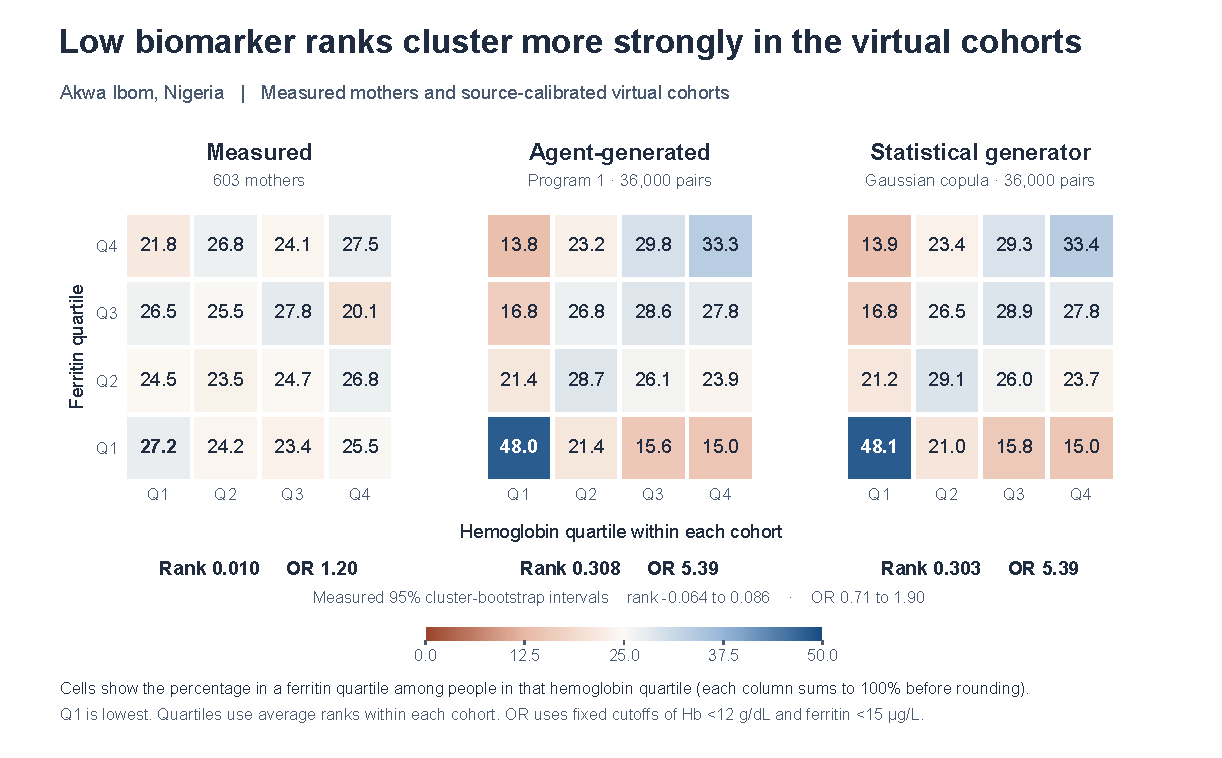
\includegraphics[width=.82\textwidth]{figures/akwa-heat.pdf}
\caption{Continuous ranks in Akwa Ibom, shown after outcome disclosure. Each cell gives the percentage in the specified ferritin quartile within a hemoglobin quartile. Quartiles are formed separately in the measured sample and each virtual law. The first prespecified agent is shown; all six have identical counts at this resolution. The odds ratios use absolute clinical cutoffs.}
\Description{Among mothers in the lowest hemoglobin quartile, the measured fraction also in the lowest ferritin quartile is 27.2 percent, compared with 48.0 and 48.1 percent in the virtual cohorts.}
\label{fig:akwa-heat}
\end{figure*}

\section{Audit of the two lipid comparisons}
\label{app:nonhdl}
The source sample was nonfasting. Mekelle used a Bio-system A25 and Haramaya a Mindray BS-200 on fasting samples. Neither cohort supplied measurements to either constructor. No reference rows were shared between the independently recruited study frames to our knowledge. The project used only the packet and no individual source records. The source mean ratio is the mean of individual ratios. For common lognormal margins, fitting the TC upper-cutoff probability allows two positive log SDs; we fixed the smaller one before generation. Each method used three seeds with 16,000 pairs per seed. Across the 48,000 records per method, HDL exceeded TC in 56 agent and 47 statistical pairs. The measured counts were zero in Mekelle and seven in Haramaya. All were retained as specified. These scientific outputs were computed after explicitly repairing the metadata interface; the raw automation had zero successful agent draws.

We resampled individuals 2,000 times within age groups 20--39 and 40 or older in each study. The 95\% intervals for the sample means were 120.19--130.00 and 120.96--126.27 mg/dL. The corresponding intervals for the fractions above or at the cutoff were 16.82--25.55\% and 18.64--23.20\%. Intervals condition on the observed age composition and frozen generators. They omit uncertainty in the original Tanzanian estimates and do not generalize the samples to the country. Among all possible permutations of the supplied empirical marginal arrays, 9.02--41.54\% can cross the threshold if no source ratio or physiological constraint is imposed. This is an outer diagnostic range for the source-constrained problem. It does not identify which assumption caused the external discrepancies.

\section{Auditing pairing decisions on frozen tables}
\label{app:pairingtest}
\paragraph{Lifestyle.} We examined all nine age- and sex-adjusted contrasts on each of the six existing tables. Conditional on the design matrix, an OLS contrast is linear in the outcomes. Under uniform joint permutation of the outcome vectors within each lifestyle-by-sex cell, its expected coefficient equals the coefficient obtained by substituting the cell means. We verified the expectation using centered within-cell covariances and exhaustive permutations on a small fixture. Real--real discrepancies are the archived mean absolute differences at matched sample size. The nine real effects were already known when this ablation was defined. The comparison measures how much this particular age pairing affected the estimate.

\paragraph{Lipids.} The protocol, source-only request, scorer, interface and budget were sealed before the four new calls. Each author received one call and had to supply a program with two scenarios. We then sealed all four programs before executing any. Each scenario used the same three ordered seeds and 16,000 observations per seed. Mean individual TC/HDL had to be within 0.02 of 3.66 on every seed and round to 3.66 in the pool. All clinical ordering constraints had to hold. Material sensitivity required a pooled difference exceeding four percentage points and a difference in the same direction exceeding two points on every seed. All four sessions met this criterion on the first call. Each marginal array had 14.4\% above the source TC cutoff and 15.3\% below the source HDL cutoff. The tariff estimate for four calls was US\$0.231. The observed seed spread measures simulation variability within a particular model pair.

\begin{figure*}[t]
\centering
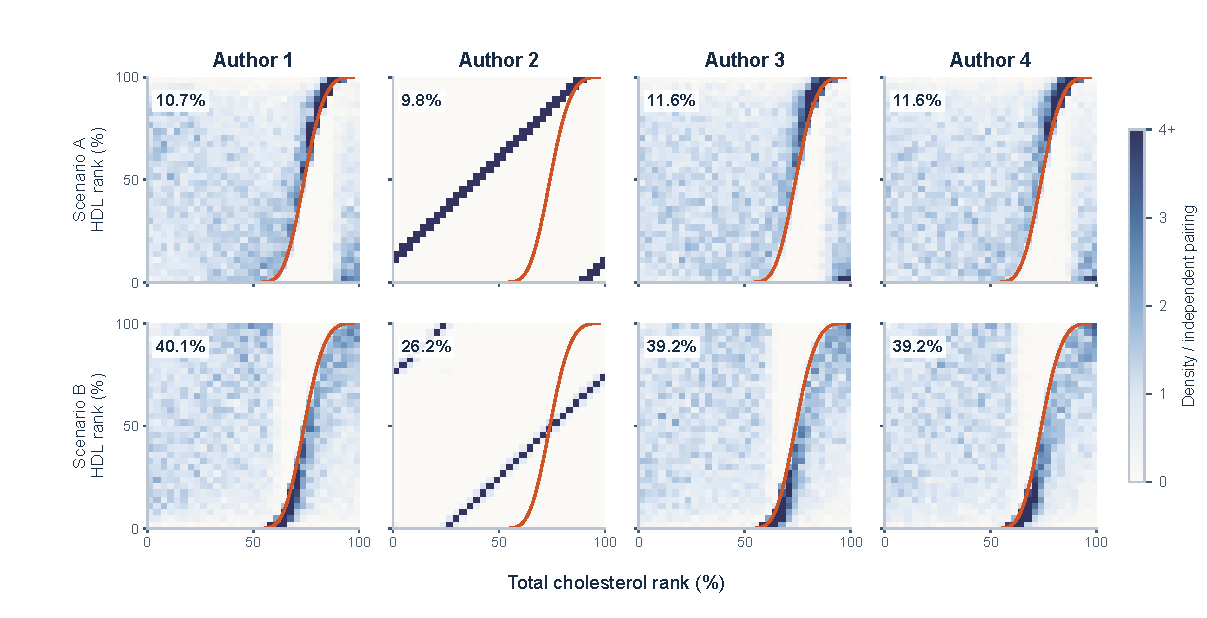
\includegraphics[width=.91\textwidth]{figures/lipid-rank-maps.pdf}
\caption{Two ways of assigning the same HDL measurements to the same total cholesterol measurements. The panels show all four authors on the first predeclared seed. Bin intensity is relative to independent rank pairing, on a common scale capped at four. Pairs below the orange curve have non-HDL at or above 160 mg/dL. Insets give the proportion from each complete draw. Author 2's rank cycles illustrate how a model can match the source ratio while imposing a distinctive joint structure.}
\Description{Eight rank density maps share the same axes. Orange curves mark the screening threshold. Opposite rank cycles are particularly visible for author two.}
\label{fig:lipidmaps}
\end{figure*}

The constructive control partitions the fixed order statistics into 125 interleaved blocks of 128. Linear assignment within each block supplies admissible permutations. Integer programming selects one per block while constraining the pooled ratio. Direct calculation on the full tables verified the two solutions. The 32.03-point spread is 98.5\% of the width of the unrestricted empirical bounds of 9.02--41.54\%. We establish two feasible points under the added conditions. The source summaries and the numerical test do not assign probabilities to the models in Figure~\ref{fig:lipidmaps}. Neither this separate four-author test nor the constructive control used another measured cohort.

\section{Prospective decisions on the Virginia sample}
\label{app:virginia}
\paragraph{Prospective decisions.}
\label{sec:virginia}
We kept the original virtual table fixed. Before opening a rural Virginia community screening study~\cite{virginiastudy,virginiadata}, eight fresh GPT sessions ranked six requested analyses. All saw the source summaries, virtual estimates, prior discrepancies in Ethiopia and a description of the new population. Four randomly assigned sessions also saw the numerical ranges from the eight agent-authored alternatives and two constructive examples. A statistical rule ranked uses by the largest available discrepancy or uncertainty relative to the intended tolerance. The rankings and unforced endorsements were sealed before we analyzed 400 adults.

\begin{figure*}[t]
\centering
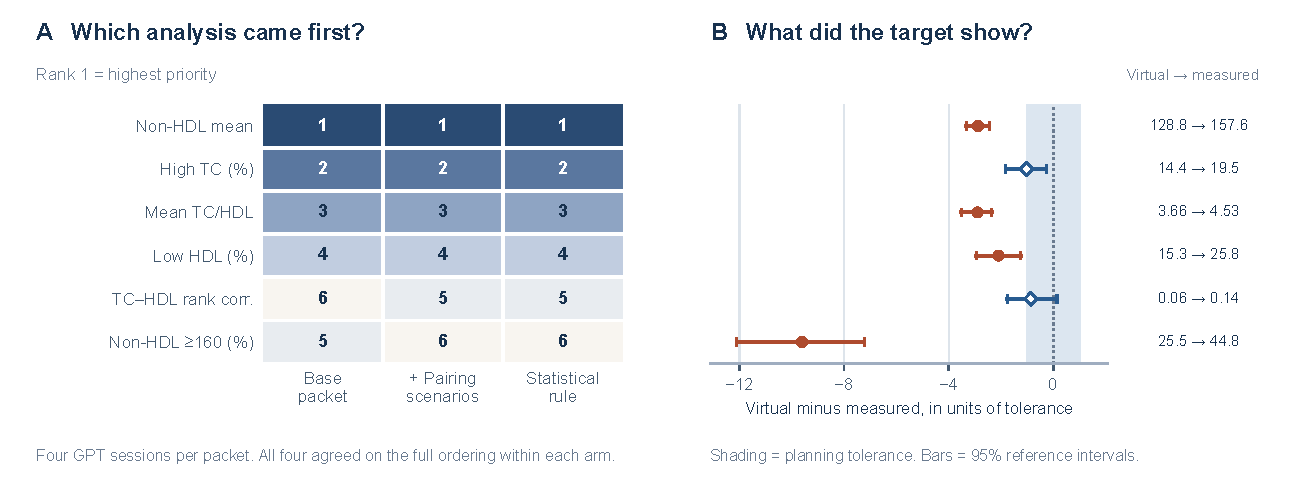
\includegraphics[width=.97\textwidth]{figures/decisions-before-disclosure.pdf}
\caption{Decisions made before access to the Virginia measurements. (A) The four advisers in each arm agreed on all six ranks. The rule received the full packet. (B) Values show the original virtual estimate and its measured counterpart. The scale is the signed difference divided by the use-specific planning tolerance. Bars are pointwise 95\% intervals from 4,000 within-county bootstrap resamples. A bar entirely within the shaded band would support that use at the declared tolerance.}
\Description{The two arms and the rule rank mean non-HDL and high TC prevalence first and second. Providing alternative pairings moves non-HDL screening from fifth to sixth. Its measured discrepancy is 9.61 tolerances. Four intervals lie outside the tolerance band and two overlap a boundary.}
\label{fig:decision}
\end{figure*}

At the primary coverage of two, all advisers and the rule chose mean non-HDL and high TC prevalence. The virtual mean was 128.77 versus 157.57 mg/dL measured, outside the $\pm10$ margin. The high-TC comparison was unresolved. Across all six uses, four intervals lay entirely outside their margins and two crossed a boundary. In the prespecified coverage curve, the arms differed only when selecting five uses. All four advisers shown alternatives set aside non-HDL screening, whose 25.53\% virtual estimate differed from 44.75\% measured by 9.61 tolerances. All four base-packet advisers set aside rank correlation instead. The statistical rule matched the full arm (Figure~\ref{fig:decision}). Seven advisers endorsed the mean when free to abstain. All eight declined to endorse the screening use.

A post-disclosure diagnostic identifies a concrete limit on revision. Across every pairing of the fixed source values the screening rate can reach at most 41.54\%. The observed Virginia rate exceeds this by 3.21 points, although its sampling interval overlaps the bound. Changing the pairing alone cannot close the observed gap at the stated two-point tolerance. The following analysis gives the margins and documents the missing second sampling frame.

\paragraph{Admission and information.}
Ten candidates were screened from study methods, participant-file documentation and prior exposure. The open Virginia study qualified for the community frame. The screened datasets for a separate type 2 diabetes frame lacked the paired biomarkers, documented subtype, individual release or independent provenance. The archive describes 403 screened participants among 1,046 rural African Americans interviewed~\cite{virginiadata,virginiastudy}. Eligibility required age at least 20, a known county and paired positive finite concentrations. The 400 eligible adults had distinct IDs, with 198 from Buckingham and 202 from Louisa. The archive's original S serialization reproduced the CSV on ID, county, age, both lipid values and the recorded ratio. All ratios for the analysis were calculated from the two component measurements. The agent saw an anonymous study description. Prior model exposure to this widely used dataset is possible. Individual fasting, assay and treatment details could not be standardized across studies.

\paragraph{Decisions and scoring.}
The full packet adds the numerical ranges of ten source-compatible alternatives to the base packet. Four randomly assigned sessions per arm used GPT-6.1 Sol at medium effort. The eight one-call response tariffs totaled US\$0.06262. The statistical rule takes the largest of three available displacements: the more distant source confidence limit from the reported point, the largest historical measured discrepancy from the fixed virtual estimate, and the largest shift under any alternative model. It scales each by the use's planning margin. Lower scores receive higher priority. A score of at most one receives an endorsement. All nine decision records were sealed before the six measured estimates were opened. We formed pointwise percentile intervals using 4,000 participant bootstrap draws stratified by county with its sample size fixed, recomputing tied ranks in each draw. Intervals compare the measured estimate to the fixed virtual table under the specified sampling assumptions.

The six margins in their original units are 10 mg/dL for mean non-HDL, 0.30 for mean individual TC/HDL, five percentage points each for high TC and low HDL, two points for non-HDL at least 160 mg/dL and 0.10 for Spearman correlation. The high-TC and low-HDL cutoffs were 6.2 and 1.0 mmol/L with respective inclusive upper-tail and strict lower-tail rules. At the original tolerance, none of the six measured intervals fit wholly within its margin. At twice the margin, the high-TC prevalence and rank correlation did. All six coverage levels and three tolerance scales were registered. The five-use illustration was selected for discussion after disclosure. The mean absolute discrepancy among those five uses was 3.70 times tolerance with the base packet and 1.95 times with alternatives. Both retained sets contained zero fully supported analyses. The two county subsets are secondary checks within one study.

\begin{figure*}[t]
\centering
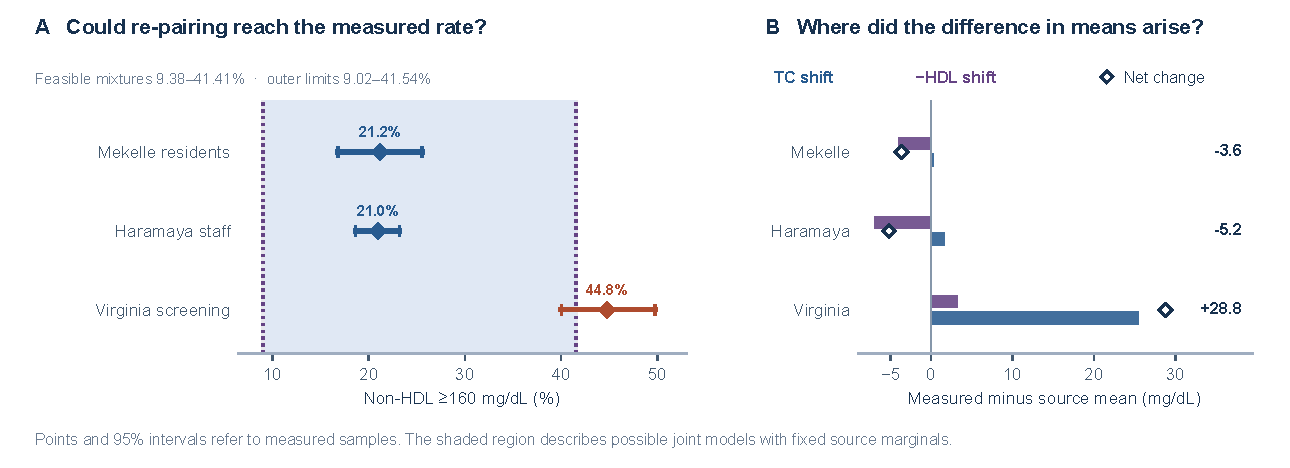
\includegraphics[width=.96\textwidth]{figures/where-pairing-can-help.pdf}
\caption{What could changing the lipid pairing correct? (A) The shaded interval contains all intermediate population-level screening fractions attainable by random mixtures of two source-compatible joint laws. Dashed lines mark the extremes over arbitrary pairings of these fixed marginal values. Measured points and intervals are shown for the two historical Ethiopian cohorts and the new Virginia study. (B) Mean non-HDL is linear in the component means. Each diamond marks the signed sum of the TC shift and the contribution of the HDL shift.}
\Description{Both Ethiopian point estimates and their intervals lie inside the achievable range. The Virginia point estimate lies outside the unrestricted upper bound while its interval overlaps. Its positive mean difference comes mostly from higher TC.}
\label{fig:repair}
\end{figure*}

\paragraph{A retrospective diagnostic for choosing the next measurement.}
For fixed empirical TC and HDL marginals, a mixture of two joint laws retains those marginals. Both the expected individual ratio and threshold probability are linear in the mixing weight. The two admissible numerical examples attain 9.375\% and 41.40625\% screening. Random mixtures attain every intermediate population-level probability and retain the accepted mean-ratio interval and component ordering. An independent count of feasible threshold matches, including ties, reproduced the unrestricted empirical limits of 9.01875\% and 41.54375\%. The resulting feasible interval spans 98.48\% of the outer width. These constructed laws carry no likelihood weights. The diagnostic was planned after the Virginia discrepancy was observed. In Ethiopia all four agent-authored scenario pairs bracketed both measured rates. In Virginia 179/400 participants crossed the threshold (44.75\%, 95\% interval 39.99--49.75\%). Its sampling interval intersects the feasible region (Figure~\ref{fig:repair}A). The 28.79 mg/dL change in mean non-HDL equals the sum of a 25.52 mg/dL rise in mean TC and a 3.28 mg/dL contribution from lower HDL, before rounding (B). Even complete knowledge of the ordering could not change that mean.

\begin{table*}[t]
\centering
\caption{Six prespecified analyses on the original lipid pairing and the same people after both historical means were adopted. Percentages and their tolerances are in percentage points. Parentheses give survey-design 95\% intervals. A use is supported when the entire interval is within its stated margin of the virtual estimate.}
\label{tab:historicalmeans}
\small
\begin{tabular}{lrrrrr}
\toprule
Analysis & Margin & Original & Updated & US 2017--2018 & US 2021--2023 \\
\midrule
Mean non-HDL (mg/dL) & 10 & 128.77 & 143.50 & 135.47 (131.87--139.06) & 135.02 (132.71--137.33)\\
Mean individual TC/HDL & 0.30 & 3.659 & 4.023 & 3.790 (3.690--3.890) & 3.732 (3.661--3.802)\\
High TC (\%) & 5 & 14.40 & 20.50 & 10.52 (8.89--12.15) & 11.21 (9.75--12.68)\\
Low HDL (\%) & 5 & 15.30 & 17.35 & 13.86 (11.53--16.20) & 11.92 (10.14--13.69)\\
Non-HDL $\geq160$ mg/dL (\%) & 2 & 25.53 & 34.25 & 25.33 (22.59--28.07) & 24.25 (22.40--26.09)\\
TC--HDL Spearman correlation & 0.10 & 0.059 & 0.059 & 0.137 (0.086--0.187) & 0.206 (0.176--0.236)\\
\bottomrule
\end{tabular}
\end{table*}

\section{Historical US information and two later survey periods}
\label{app:historicalmeans}
Mwanza reported the mean of the ratios formed within individuals (3.66) alongside the separate marker means and frequencies~\cite{kavishe}. Our historical US inputs were the 2007--2010 entries in Table~1 of Carroll et al.~\cite{carroll_history}, for adults aged 20 or older of both sexes (11,028 participants). The reported age-standardized 95\% intervals were 195--198 mg/dL for TC and 51.8--53.2 for HDL. These inputs contain no target-period joint threshold or mean individual ratio. The four authors, the proportional rule and the original model were evaluated under all nine frozen pairings. The three seeds within each pairing approximate its sampling law. All new authors used the same model and chose the same numerical transformation. Independent parsing, scoring and seed-level checks reproduced all 54 method-by-pairing combinations.

The US comparison retained adults aged 20 or older with both markers, including those taking lipid-lowering medication. We used the examination weight for 2017--2018 and the phlebotomy weight for August 2021--August 2023~\cite{cdc_lipids_l}. We directly standardized to the US year-2000 adult age distribution (20--39, 40--59 and 60+). Each of 15 masked strata contributed two primary sampling units per wave. We restandardized after each stratified delete-one-unit jackknife replicate and formed two-sided intervals using 15 degrees of freedom. The intervals quantify measured-sample variation conditional on the sealed virtual predictions. Both periods are later waves of the same survey family as the historical source.



The primary decision required a reduction of at least two percentage points in median author absolute screening error in both periods on the original pairing. Before disclosure, the screening rate at which the original and updated predictions would be equally close was 29.89\%. Both measured intervals fell below this point. Over these intervals the gain ranged from $-8.72$ to $-3.63$ and from $-8.72$ to $-7.59$ points respectively. Although the original screening predictions were close to both measured points, their intervals crossed the two-point use margin. Table~\ref{tab:historicalmeans} reports the five secondary analyses on exactly the same records. The high-TC and low-HDL cutoffs were $\geq6.2$ and $<1.0$ mmol/L respectively.

\paragraph{Which virtual participants crossed the threshold?}
Each update multiplied TC by $a=1.07384$ and HDL by $b=0.97672$. A participant previously below 160 mg/dL crossed exactly when the original TC lay in $[(160+b\,\mathrm{HDL})/a,\,160+\mathrm{HDL})$. A separate count reproduced every change in prevalence at each seed. From 0.36\% to 26.34\% of virtual participants crossed under the eight alternatives. All eight were prespecified. Grouping the alternatives by their original screening rate and tracing individual crossings were retrospective explanations. Across both entire survey intervals, one of the four initially lower scenarios improved and all four initially higher scenarios worsened. The arithmetical consequences differ by analysis. The mean individual ratio is multiplied by $a/b$ (a 9.94\% rise), the rank correlation is invariant, and the updated mean non-HDL is the difference between the two historical means. The four methods' common choice to preserve shape leaves other marginal transformations unevaluated.

\section{Bilateral grip and three recruitment settings}
\label{app:grip}
\paragraph{Information and scientific uses.}
Massy-Westropp et al.~\cite{grip_adelaide} published anatomical right and left means and SDs in four strata (men and women aged 50--59 and 60--69). Their seated protocol averages three Jamar trials and excludes participants with hand pain or arthritis. We gave each stratum equal weight, constructed positive normal quantile grids rescaled to its two means and SDs, and fixed all 4,096 values for each hand in each cell. Four marginal-only (M) and four joint-evidence (J) sessions used the same GPT-6.1 Sol configuration. J also received the mean (0.9534) and SD (0.1100) of individual nondominant-to-dominant ratios from Wunderle et al.~\cite{grip_ratio}. That study pooled 444 non-left-handed adults across ages and sexes, using a pressure device. The instrument, definition of hand, and population all differ from the Australian report.

\begin{table*}[t]
\caption{Four scientific uses of the same handgrip records. Square brackets give pointwise 95\% measured-sample intervals. A virtual range covers the four J authors; all four M authors produced a single assignment for each seed. The planning margins were 1 kg, 5 percentage points, 2 kg and 0.10, respectively.}
\label{tab:grip}
\centering\small
\begin{tabular}{lrrrr}\toprule
Setting or construction & Mean absolute gap (kg) & Gap $\geq$5 kg (\%) & Mean of both hands (kg) & Rank correlation\\\midrule
US NHANES ($n=1{,}423$) & 3.30 [3.07, 3.52] & 20.95 [17.49, 24.40] & 33.11 [32.26, 33.96] & .801 [.751, .851]\\
South Africa HAALSI ($n=2{,}434$) & 3.78 [3.52, 4.05] & 27.71 [25.00, 30.42] & 25.57 [25.01, 26.12] & .756 [.718, .794]\\
Rio Branco maximum ($n=464$) & 3.22 [2.89, 3.55] & 26.99 [21.99, 32.00] & 29.93 [29.04, 30.82] & .824 [.783, .865]\\\midrule
M authors & 3.814 & 28.94 & 33.375 & .784\\
J authors & 3.371--3.413 & 23.40--23.53 & 33.375 & .837--.839\\
Ratio-based statistical model & 3.424 & 23.75 & 33.375 & .836\\
Independent pairing (expectation) & 7.932 & 60.24 & 33.375 & .000\\\bottomrule
\end{tabular}
\end{table*}

\paragraph{Prospective paired measurements.}
The US NHANES 2011--2012 examination~\cite{grip_cdc} gives randomized starting hand, bilateral trials and effort flags. We required maximal effort on the first two trials for each hand and a positive examination weight. HAALSI baseline v3~\cite{grip_haalsi} supplied two cleaned measurements for each anatomical hand in rural Agincourt. We used the within-hand trial mean in both main settings. The separate Rio Branco study~\cite{grip_rio} released only the maximum per hand. We required both upper limbs to be eligible in that dataset. All settings weighted the four sex-by-decade cells equally. Within cells we used the US examination weights, Rio survey weights and equal weights in Agincourt. Pointwise intervals use a delete-one-cluster jackknife and $t$ quantiles with 17, 26 and 78 design degrees of freedom in the US, South Africa and Brazil. Rank correlation is the equally weighted average of within-cell weighted Spearman correlations. The Brazilian study was designated as a measurement stress test before scoring. The investigator had seen ancillary single-hand descriptions during admission. Both main survey families had appeared in other analyses. Constructors received no target participant measurements, single-hand summaries or paired estimates.

\paragraph{What did the additional evidence change?}
Three J programs derived dependence from ratio dispersion; one used 0.85 as a working correlation. The statistical rule estimated a within-cell correlation from the marginal coefficients of variation and the variance of log ratio, then paired ranks with a Gaussian copula. This rule shares J's indirect analogy between a pooled German pressure ratio and anatomical force ratios. The four independent M sessions returned distinct code but identical assignments for every shared seed. J returned four distinct assignments. Each of the eight programs generated 16,384 records at each of three seeds. The recorded tariff estimate for the eight completions was US\$0.2622.

Table~\ref{tab:grip} reports all observed uses. The US and South African point gains of 4.12 kg relative to independent pairing coincide because both measured mean gaps fall below both predictions. Holding the virtual outputs fixed, the mean-gap improvement from M to the median J author ranged from $+0.16$ to $+0.43$ kg across the US reference interval, and from $-0.43$ to $+0.16$ kg across South Africa's. At their respective measured points the gains were $+0.43$ and $-0.37$ kg. In Brazil the point gain was $+0.43$ kg. The same-evidence statistical rule was within 0.05 kg of the median J absolute error at every measured point.

\paragraph{What else could the source have supported?}
Holding the finite Australian grids fixed, pairing the order statistics in the same or reversed order gives the exact minimum and maximum possible mean gaps, 1.75 and 11.12 kg. This follows from the two-pair exchange inequality for absolute distance. In a retrospective continuous Gaussian calculation, common within-cell correlations from 0.762 to 0.883 place the virtual estimate within 1 kg over both complete principal reference intervals (Figure~\ref{fig:gripsens}). No new author, participant draw or coefficient fit enters this calculation. A separate prespecified diagnostic replaced the Australian marginals with each target's two separate empirical quantile grids and kept the archived permutations. M's mean gaps became 3.60, 3.97 and 3.97 kg in the US, South Africa and Brazil. The bilateral means then agreed within 0.002 kg by construction. This same-sample diagnostic illustrates how improving the overall marker levels can leave the between-hand discrepancy larger.

\begin{figure}[t]
\centering
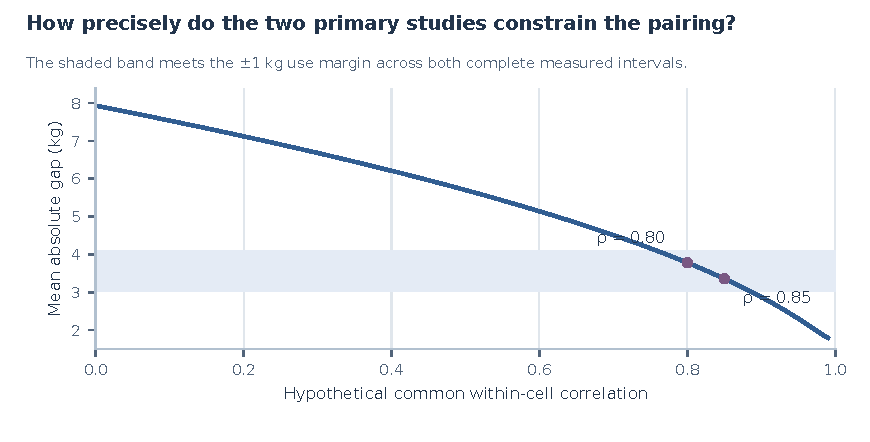
\includegraphics[width=.99\columnwidth]{figures/grip-correlation-sensitivity.pdf}
\caption{Retrospective sensitivity of the expected gap to a common within-group correlation under continuous normal single-hand distributions. The shaded band includes virtual gap estimates within 1 kg over both primary measured intervals.}
\Description{A curve slopes down from 7.93 kg at zero correlation to 1.75 kg near perfect correlation. The virtual mean gap is inside the shaded band for correlations of approximately 0.762 to 0.883.}
\label{fig:gripsens}
\end{figure}

\end{document}
